\section{Desempeño para distintos conjuntos de predictores}

Se analizó el rendimiento de la red neuronal para el pronóstico de precipitación para la región específica de Bocacosta, mediante las métricas de validación en el entrenamiento. Comparando cada uno de los conjuntos de predictores numerados en la subsección \ref{subsec:fuentes_de_datos}, con el objetivo de encontrar la mejor combinación posible para un adecuado pronóstico. Los resultados fueron los siguientes:
\begin{figure}[H]
    \centering
    
\includegraphics[width=14.0 cm]{Informe/resultados/comparacion_combinaciones.png}
    \caption{Comparación de métricas para distintos predictores}
    \label{fig:comparación_combinaciones}
\end{figure}
\begin{figure}[H]
    \centering
    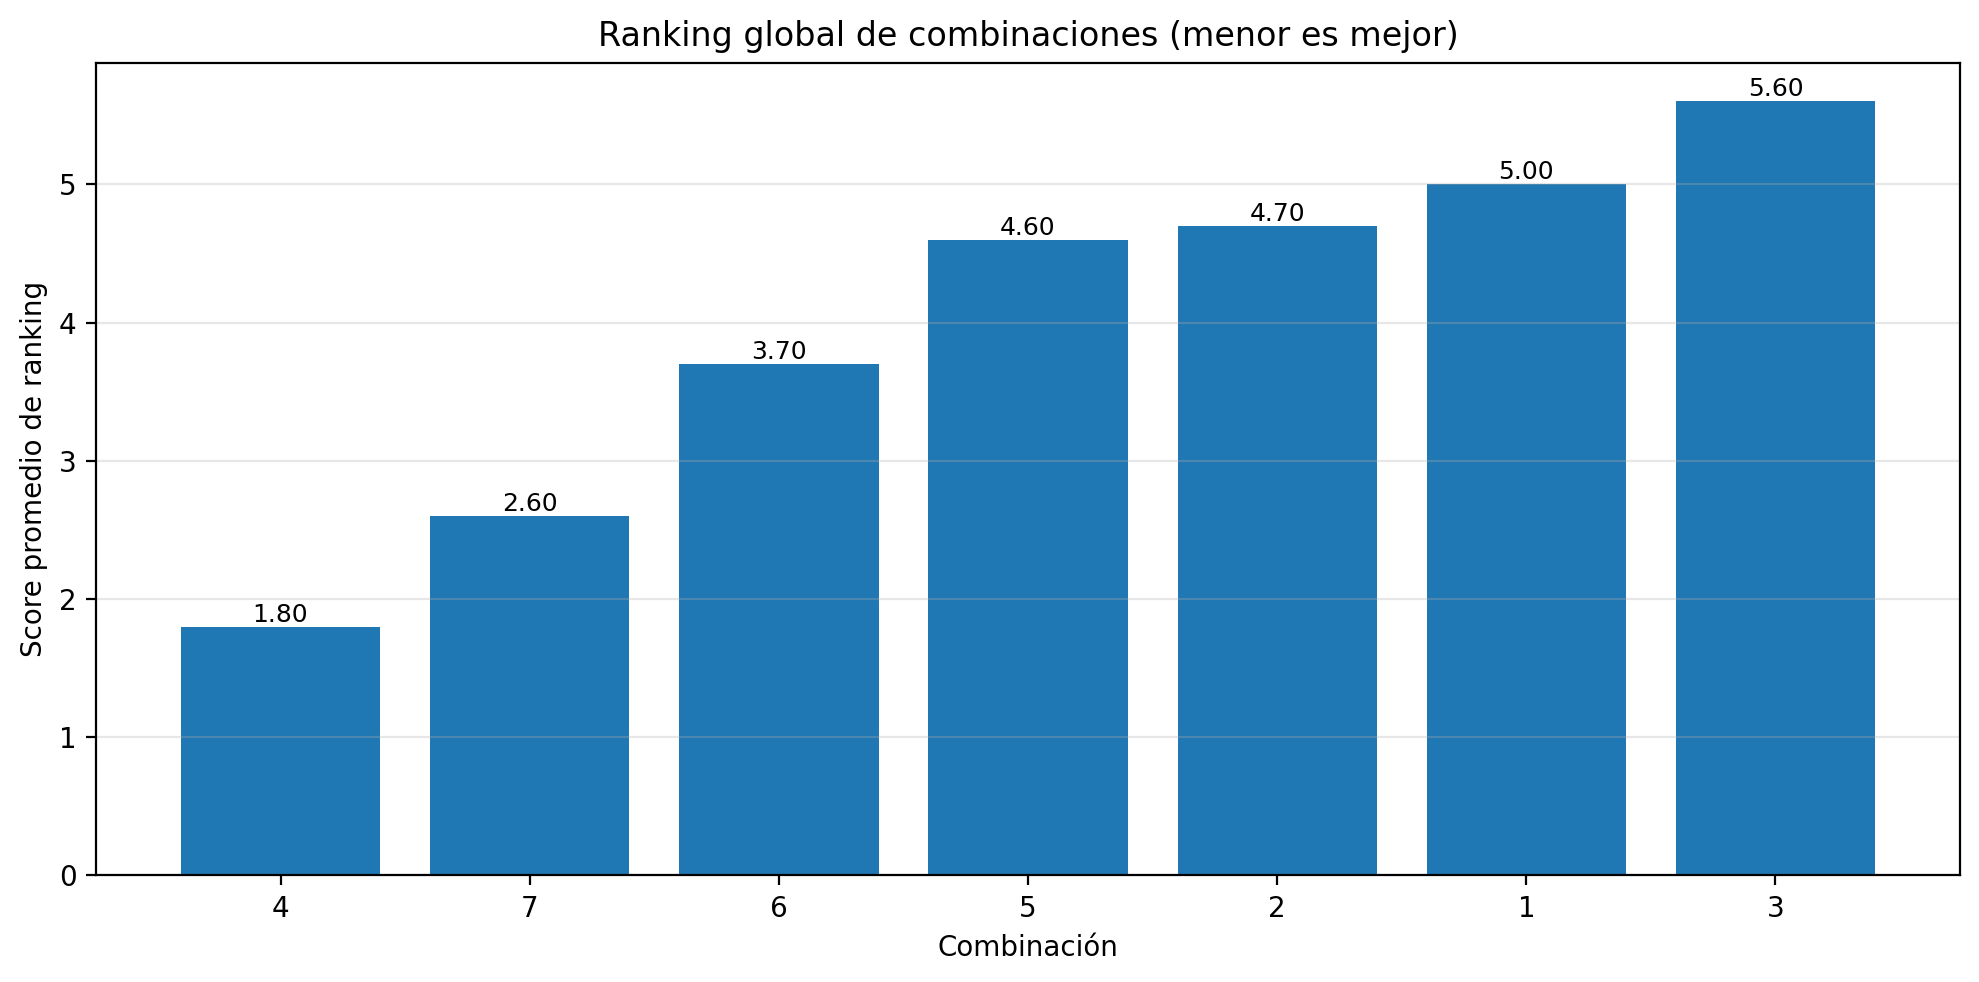
\includegraphics[width=14.0 cm]{Informe/resultados/ranking_combinaciones.png}
    \caption{Los resultados muestran que la combinación óptima de predictores fue: SST, tp y MJO.}
    \label{fig:comparación_combinaciones}
\end{figure}

En donde el \textit{score promedio} es un promedio de rankings multi-métrica, donde todas las métricas pesan igual y el objetivo es minimizar ese promedio. Así, la combinación 4 resultó ser la más eficaz, es decir, SST, tp y MJO. Se entrenó el modelo con esta combinación para hacer el análisis de pronósticos de las secciones posteriores.

\section{Métricas de validación para el territorio nacional}\label{sec:métricas de validación}

Se obtuvieron los siguientes resultados para toda la región guatemalteca, para la validación de un entrenamiento considerado desde el 1 de enero de 1981 hasta el 31 de diciembre de 2024:
\scriptsize
\begin{verbatim}
    Estadísticas globales
  RMSE                      = 80.5953
  MAE                       = 56.0282
  Bias (media)              = -0.2901
  % Bias                    = -0.19 %
  Std(error)                = 80.5948
  R²                        = 0.6348
  Pearson r                 = 0.7979  (p=0.00e+00)
  Spearman                  = 0.8431  (p=0.00e+00)
  Nash-Sutcliffe            = 0.6348
  Kling-Gupta (KGE)         = 0.7435
  
    Métricas por mes
  Mes    RMSE    MAE    Bias     r   NSE   KGE
  Ene  55.120 36.127 -20.822 0.765 0.511 0.532
  Feb  34.379 22.299  14.362 0.761 0.250 0.500
  Mar  33.291 21.433   5.791 0.578 0.227 0.526
  Abr  50.620 36.736   2.151 0.386 0.013 0.337
  May  89.026 64.347 -23.209 0.626 0.347 0.456
  Jun  97.403 76.168   7.719 0.590 0.311 0.529
  Jul 112.017 86.955  41.622 0.653 0.333 0.442
  Ago  99.861 72.419 -11.995 0.726 0.491 0.475
  Sep 106.291 80.194 -40.323 0.548 0.155 0.440
  Oct  92.504 72.770  20.551 0.592 0.293 0.506
  Nov  74.127 54.606  -6.837 0.668 0.434 0.584
  Dic  64.787 44.968   4.088 0.597 0.273 0.575

    Análisis de extremos (percentiles)
  P90 (>= 331.1 mm): n=28187, r=0.381, RMSE=161.9, Bias=-118.8
  P95 (>= 406.6 mm): n=14094, r=0.326, RMSE=201.4, Bias=-165.4
  P99 (>= 572.9 mm): n=2819, r=0.229, RMSE=317.1, Bias=-289.3
  
    Percentiles cruzados
  P10  obs=   11.75   pred=   14.42   ratio=1.227
  P25  obs=   43.34   pred=   54.59   ratio=1.260
  P50  obs=  121.64   pred=  135.64   ratio=1.115
  P75  obs=  222.12   pred=  226.93   ratio=1.022
  P90  obs=  331.13   pred=  307.85   ratio=0.930
  P95  obs=  406.58   pred=  355.25   ratio=0.874
\end{verbatim}
\normalsize

En donde la eficiencia del modelo en los píxeles del mapa queda representada como sigue:
\begin{figure}[H]
    \centering
    
\includegraphics[height=5.0 cm]{Informe/resultados/Guatemala/13_nse_kge_mapa.png}
    \caption{NSE y KGE para el territorio nacional en los datos de validación del entrenamiento.}
    \label{fig:Informe/resultados/Guatemala/13_nse_kge_mapa}
\end{figure}
\begin{figure}[H]
    \centering
    
\includegraphics[height=4.0 cm]{Informe/resultados/Guatemala/03_mapas_metricas.png}
    \caption{Sesgo medio, RMSE y correlación de Pearson para el territorio nacional en los datos de validación del entrenamiento.}
    \label{fig:Informe/resultados/Guatemala/03_mapas_metricas}
\end{figure}

Las métricas mensuales y el ciclo anual medio obtenidos fueron los siguientes:
\begin{figure}[H]
    \centering
    
\includegraphics[height=7.0 cm]{Informe/resultados/Guatemala/06_metricas_mes.png}
    \caption{RMSE, sesgo medio, correlación de Pearson y coeficiente de Kling-Gupta mensuales medios para los datos de validación del entrenamiento.}
    \label{fig:Informe/resultados/Guatemala/06_metricas_mes}
\end{figure}

\begin{figure}[H]
    \centering
    
\includegraphics[height=5.0 cm]{Informe/resultados/Guatemala/05_ciclo_anual.png}
    \caption{Precipitación media mensual para los datos de validación del entrenamiento en el territorio nacional.}
    \label{fig:Informe/resultados/Guatemala/05_ciclo_anual}
\end{figure}

\section{Métricas de validación para la región de Bocacosta}

En particular, para la región de Bocacosta se obtuvo que:
\scriptsize
\begin{verbatim}
    Estadísticas globales
  RMSE                      = 110.4970
  MAE                       = 74.6254
  Bias (media)              = -12.9062
  % Bias                    = -6.13 %
  Std(error)                = 109.7406
  R²                        = 0.6814
  Pearson r                 = 0.8281  (p=0.00e+00)
  Spearman                  = 0.8636  (p=0.00e+00)
  Nash-Sutcliffe            = 0.6814
  Kling-Gupta (KGE)         = 0.7524

    Métricas por mes
Mes    RMSE     MAE    Bias     r    NSE    KGE
Ene  22.982  15.408 -10.469 0.292 -0.156 -0.147
Feb  14.137  10.177   3.708 0.083 -0.656 -0.039
Mar  40.034  26.093  -6.367 0.145 -0.238  0.046
Abr  95.424  75.495   6.043 0.095 -0.259  0.013
May 175.586 114.414 -89.871 0.458 -0.071  0.206
Jun 110.029  89.730  -7.688 0.510  0.237  0.397
Jul 134.683 113.894 107.037 0.443 -1.510  0.233
Ago 164.154 129.000 -13.728 0.562  0.261  0.207
Sep 149.160 118.770 -59.664 0.198 -0.328  0.089
Oct 111.057  90.556 -47.196 0.530  0.114  0.381
Nov  97.630  76.933 -25.384 0.223 -0.069  0.018
Dic  31.536  25.165 -10.888 0.171 -0.200 -0.035

    Análisis de extremos (percentiles)
  P90 (>= 486.9 mm): n=1726, r=0.103, RMSE=241.4, Bias=-203.8
  P95 (>= 570.8 mm): n=863, r=0.036, RMSE=300.5, Bias=-270.5
  P99 (>= 746.7 mm): n=173, r=-0.147, RMSE=454.4, Bias=-437.1
  
    Percentiles cruzados
  P10  obs=    5.03   pred=    9.03   ratio=1.793
  P25  obs=   29.46   pred=   24.44   ratio=0.830
  P50  obs=  169.16   pred=  199.29   ratio=1.178
  P75  obs=  346.15   pred=  338.45   ratio=0.978
  P90  obs=  486.88   pred=  416.63   ratio=0.856
  P95  obs=  570.84   pred=  455.79   ratio=0.798
\end{verbatim}
\normalsize

Las métricas mensuales y el ciclo anual medio obtenidos fueron los siguientes:
\begin{figure}[H]
    \centering
    
\includegraphics[height=7.0 cm]{Informe/resultados/Bocacosta/06_metricas_mes.png}
    \caption{RMSE, sesgo medio, correlación de Pearson y coeficiente de Kling-Gupta mensuales medios para los datos de validación del entrenamiento en la región de Bocacosta.}
    \label{fig:Informe/resultados/Bocacosta/06_metricas_mes}
\end{figure}

\begin{figure}[H]
    \centering
    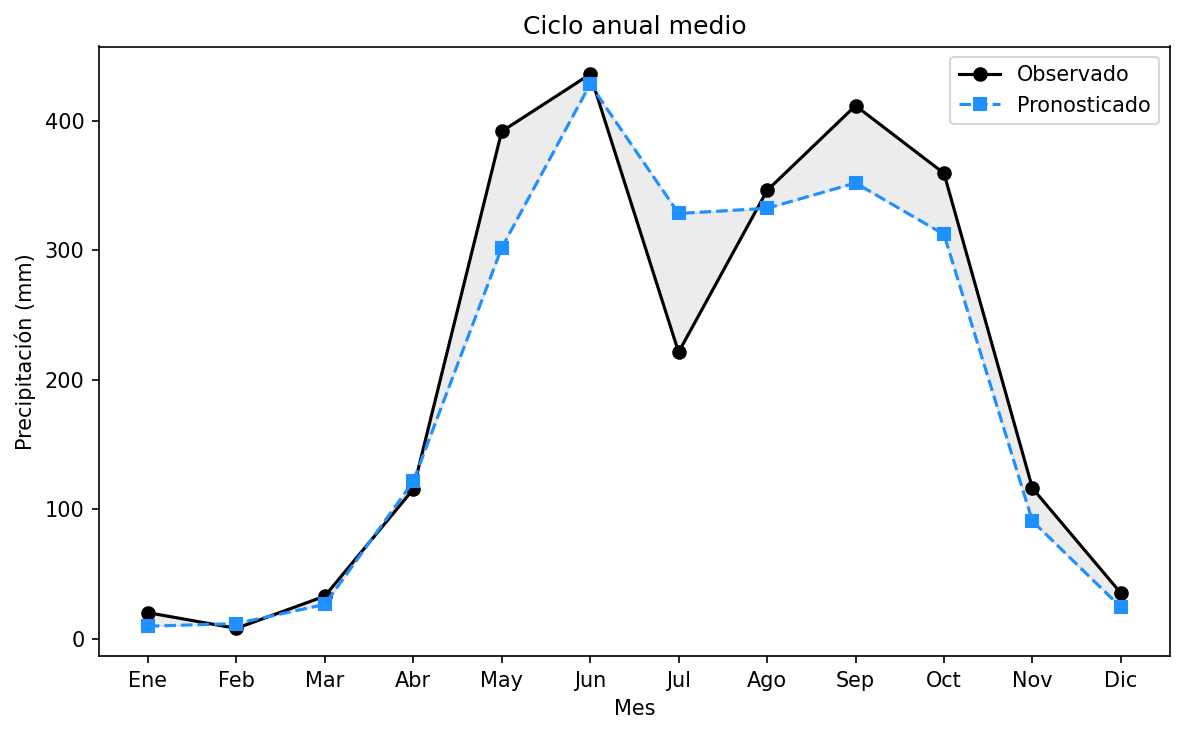
\includegraphics[height=5.0 cm]{Informe/resultados/Bocacosta/05_ciclo_anual.png}
    \caption{Precipitación media mensual para los datos de validación del entrenamiento en la región de Bocacosta.}
    \label{fig:Informe/resultados/Bocacosta/05_ciclo_anual}
\end{figure}

\section{Comparación con el método}



\section{Comparación con la precipitación real del año 2025}

Se utilizó el modelo entrenado en la sección \ref{sec:métricas de validación} para pronosticar todos los meses del 2025, utilizando por tanto, los predictores de SST, TP; RMM1 y RMM2 de las MJO de treinta y un días previos al mes objetivo, y se obtuvieron los siguientes resultados:

% ========================= ENERO =========================
\begin{figure}[H]
    \centering
    % Primera subfigura
    \begin{subfigure}[b]{0.45\textwidth}
        
\includegraphics[width=\textwidth]{Informe/resultados/pronósticos/Pronóstico_1_2025_Boca Costa_03.png}
        \caption{Pronóstico de precipitación acumulada para el mes de enero de 2025 dado por la LSTM.}
        \label{fig:pronosticolstm2501}
    \end{subfigure}
    \hfill
    % Segunda subfigura
    \begin{subfigure}[b]{0.45\textwidth}
        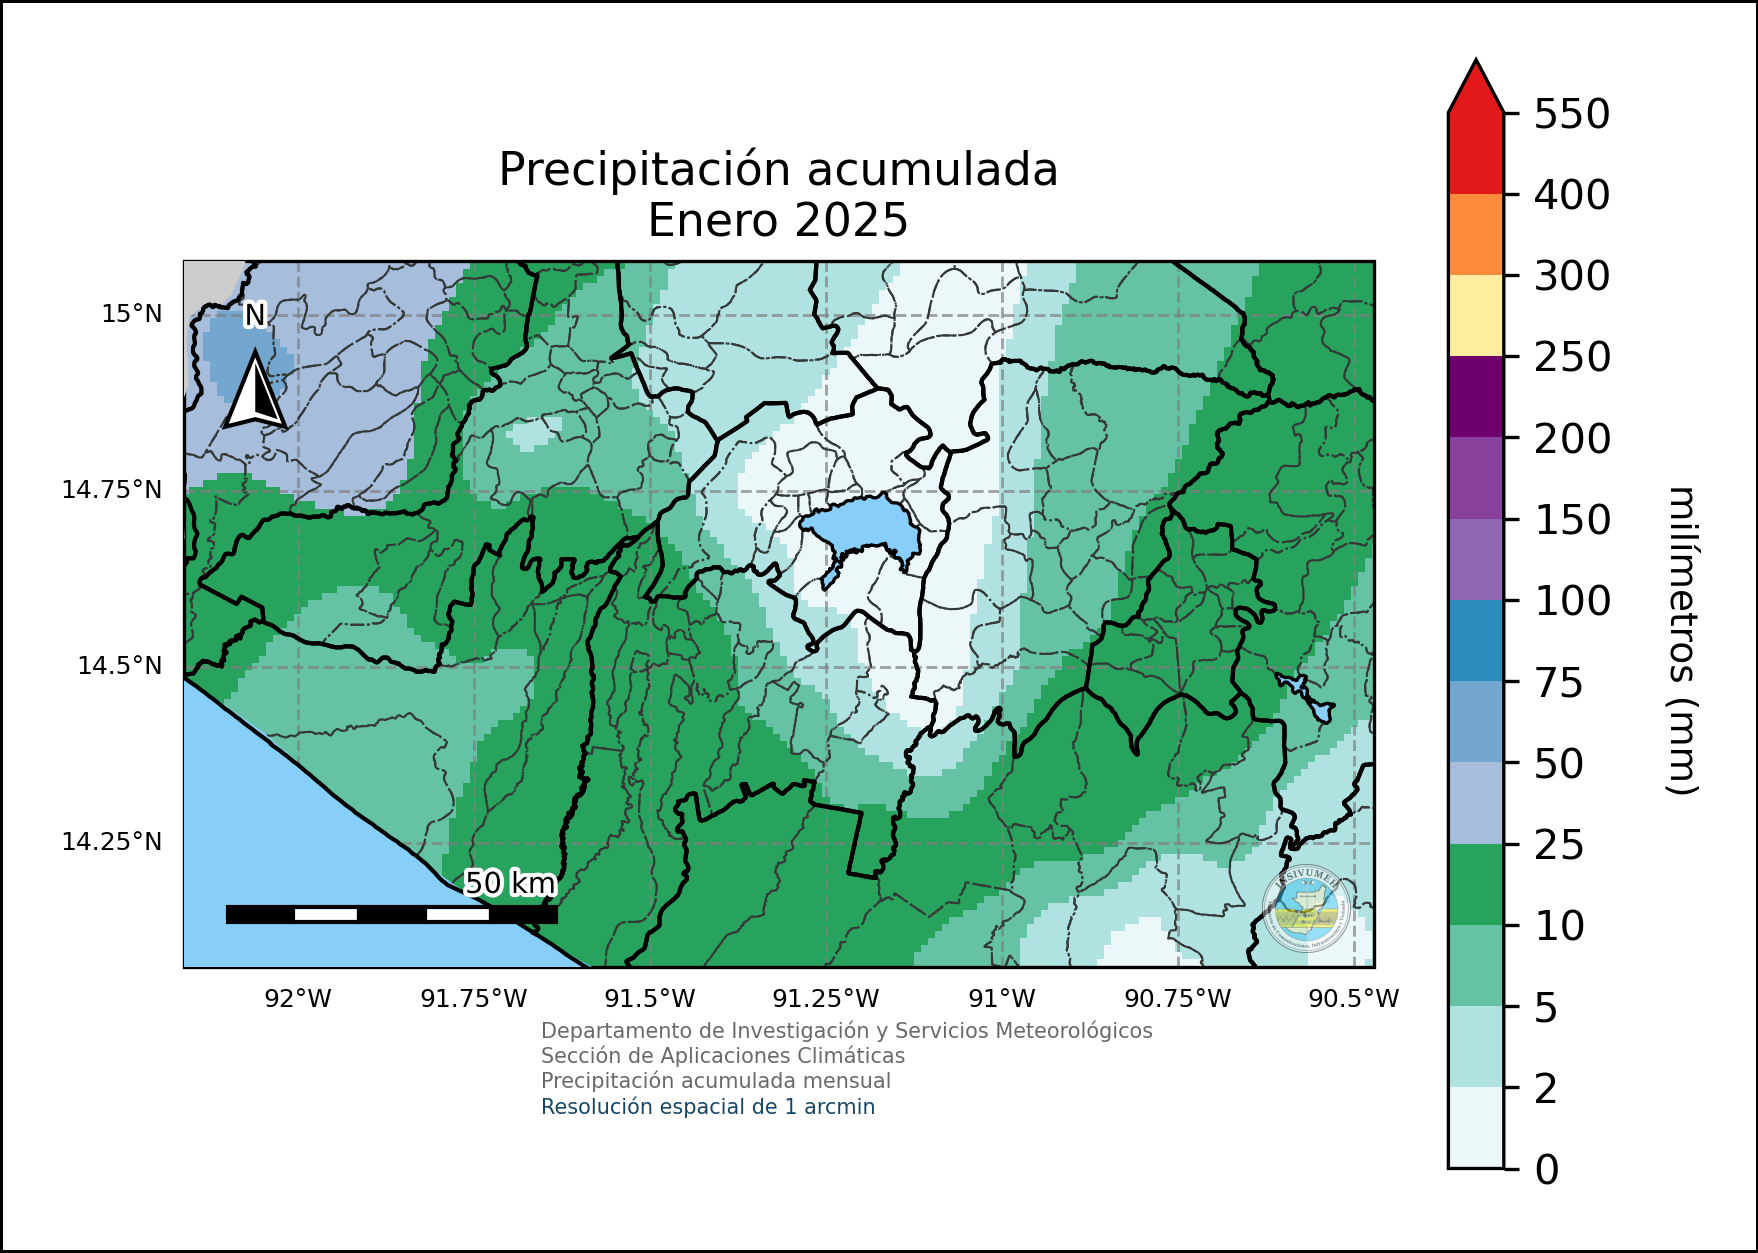
\includegraphics[width=\textwidth]{Informe/resultados/precipitación/Precipitación_1_2025_Boca Costa_03.png}
        \caption{Precipitación acumulada para el mes de enero de 2025 dado por el registro de datos ENACTS.}
        \label{fig:precipenacts2501}
    \end{subfigure}
\end{figure}

% ========================= FEBRERO =========================
\begin{figure}[H]
    \centering
    \begin{subfigure}[b]{0.45\textwidth}
        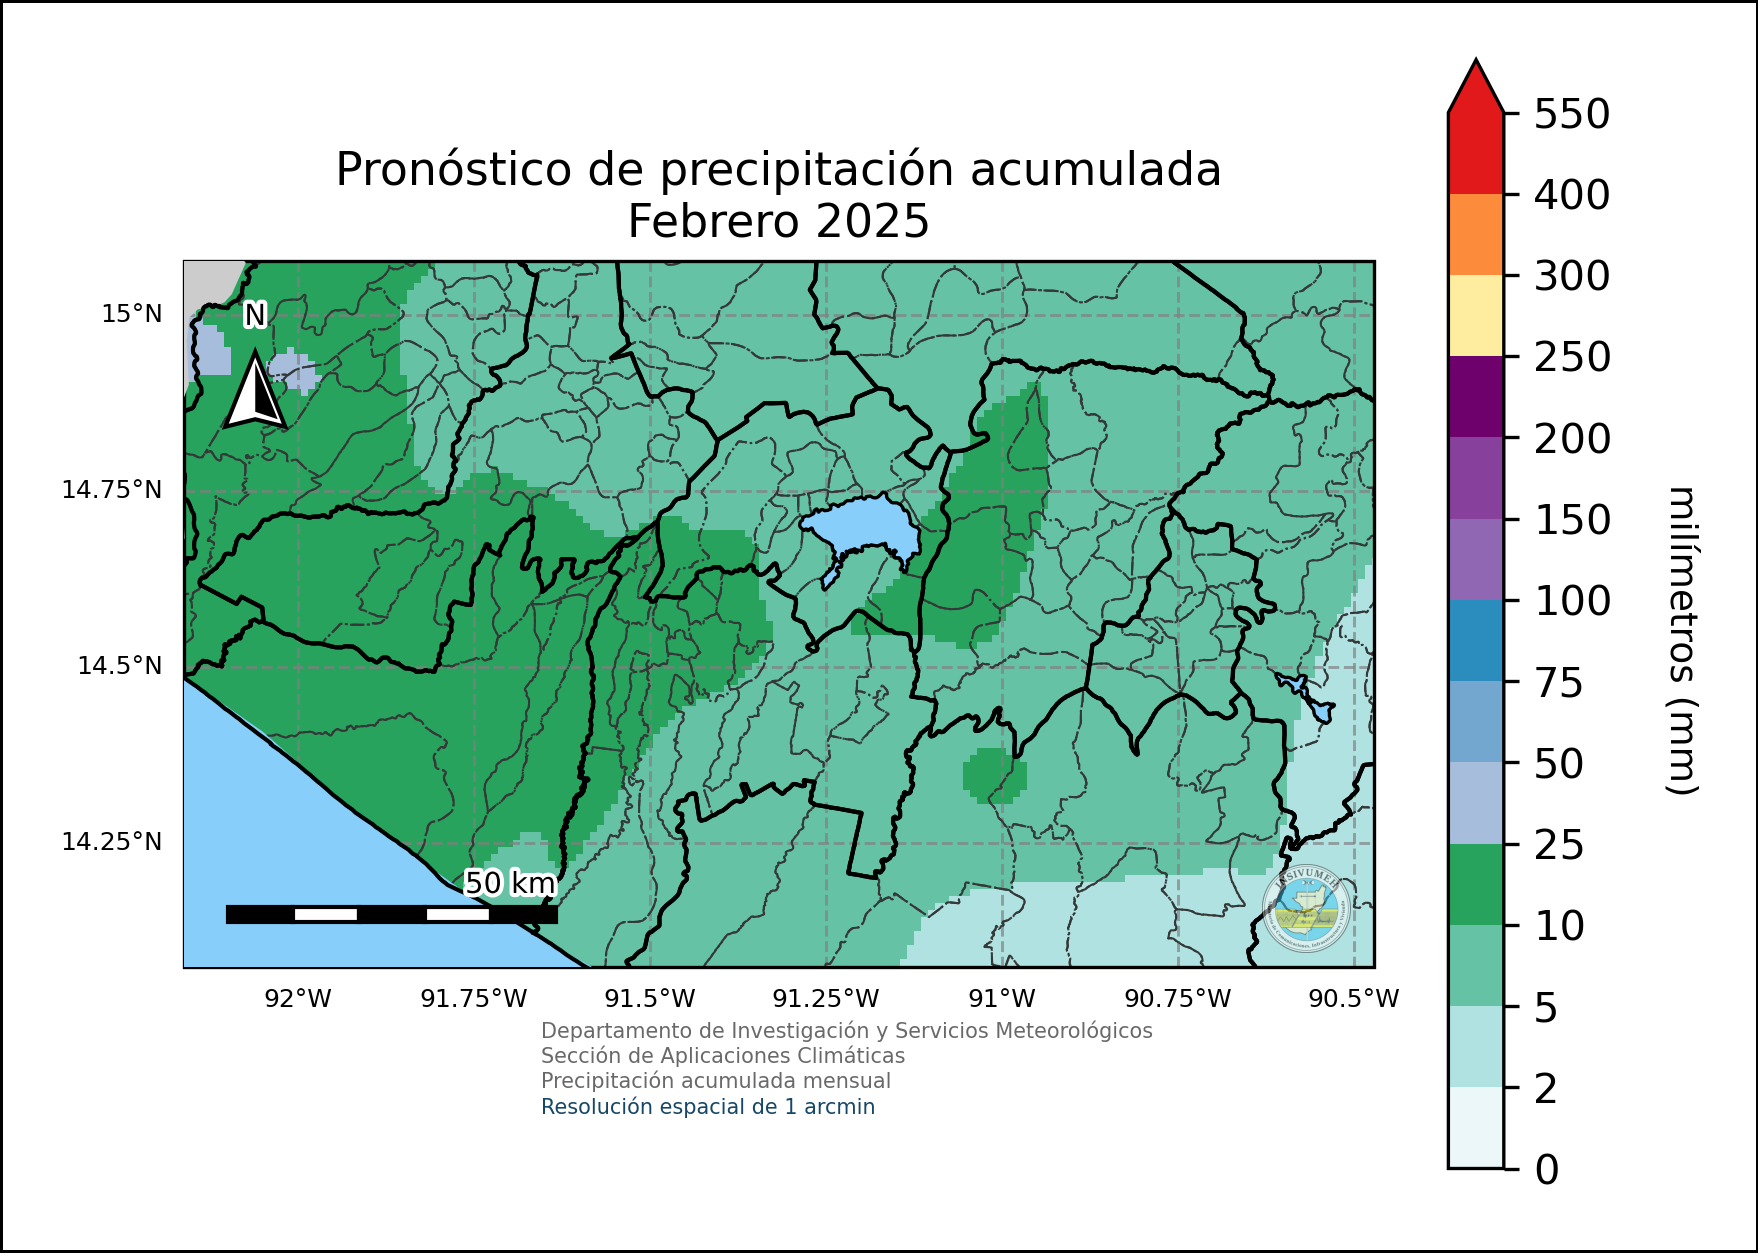
\includegraphics[width=\textwidth]{Informe/resultados/pronósticos/Pronóstico_2_2025_Boca Costa_03.png}
        \caption{Pronóstico de precipitación acumulada para el mes de febrero de 2025 dado por la LSTM.}
        \label{fig:pronosticolstm2502}
    \end{subfigure}
    \hfill
    \begin{subfigure}[b]{0.45\textwidth}
        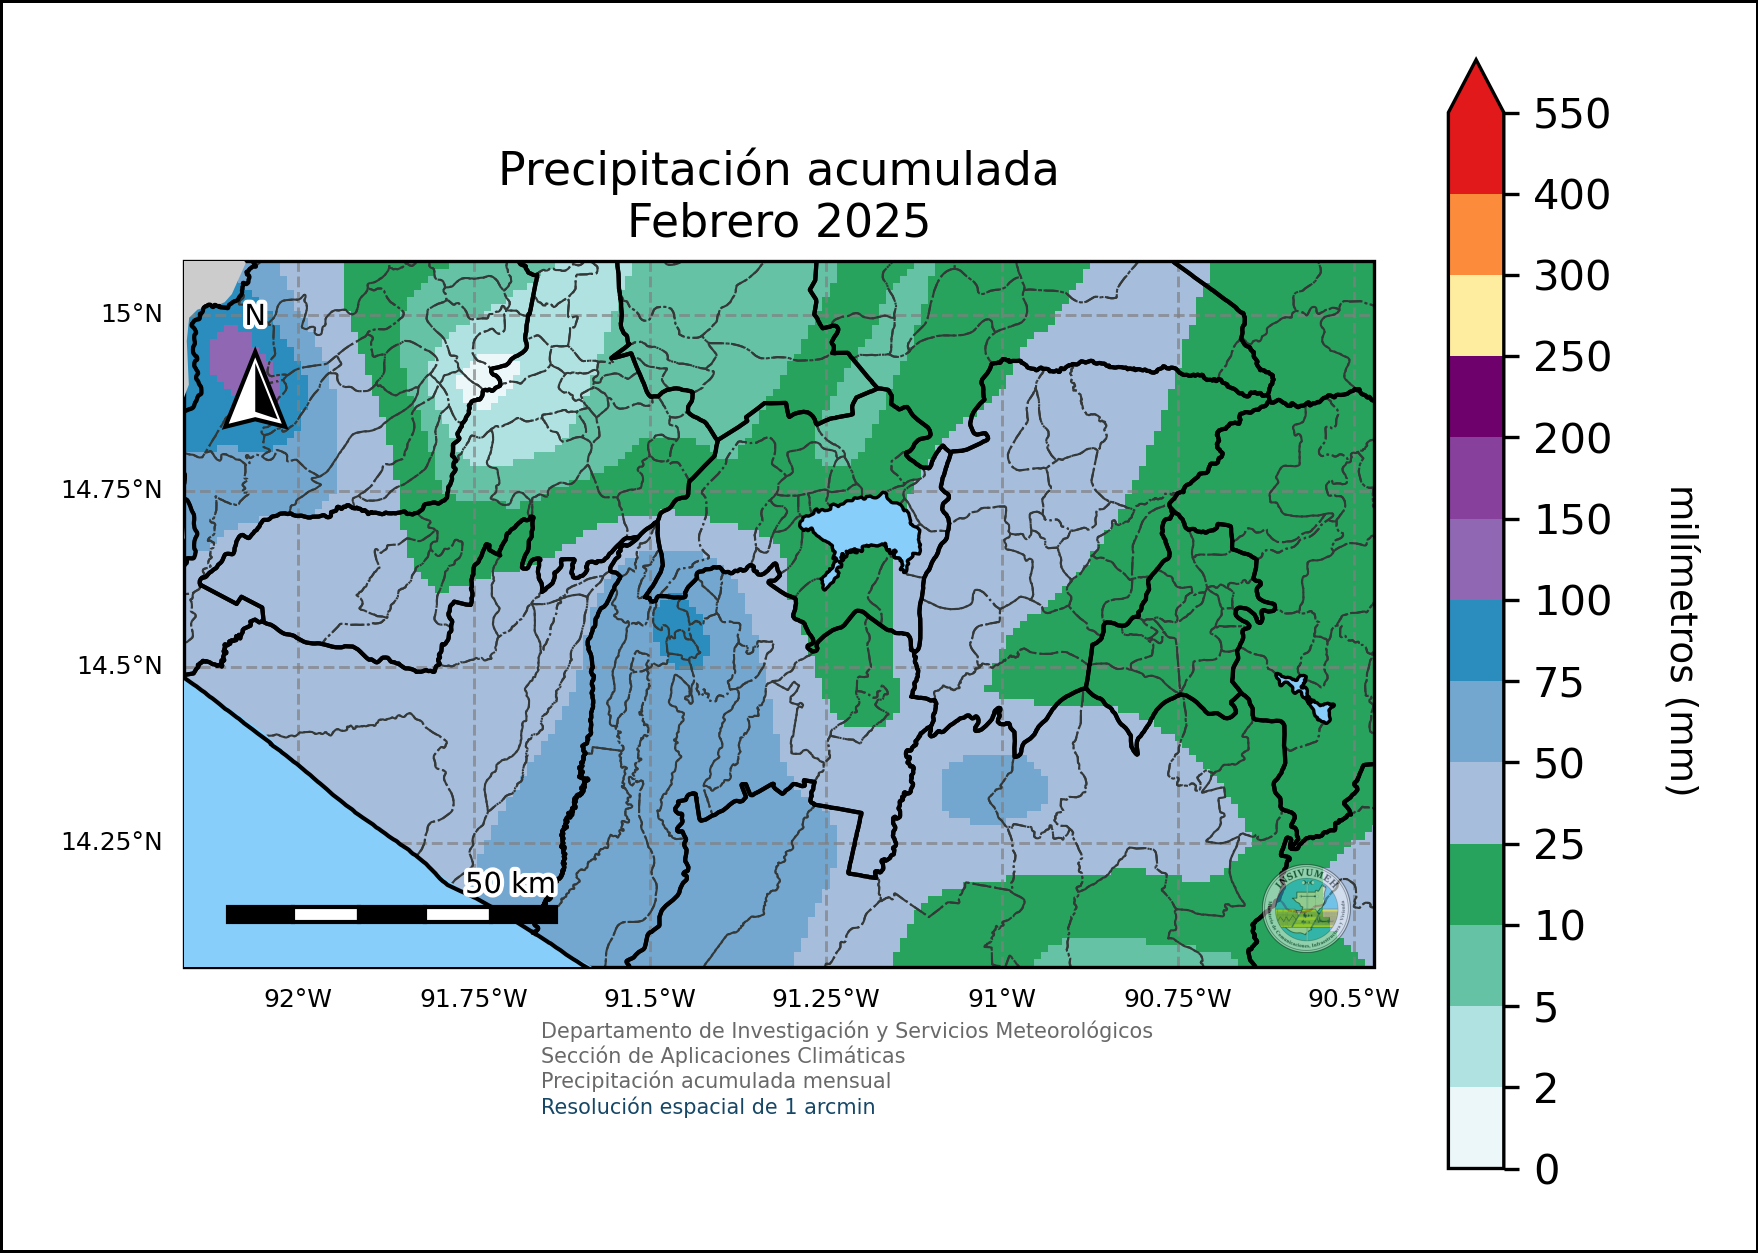
\includegraphics[width=\textwidth]{Informe/resultados/precipitación/Precipitación_2_2025_Boca Costa_03.png}
        \caption{Precipitación acumulada para el mes de febrero de 2025 dado por el registro de datos ENACTS.}
        \label{fig:precipenacts2502}
    \end{subfigure}
\end{figure}

% ========================= MARZO =========================
\begin{figure}[H]
    \centering
    \begin{subfigure}[b]{0.45\textwidth}
        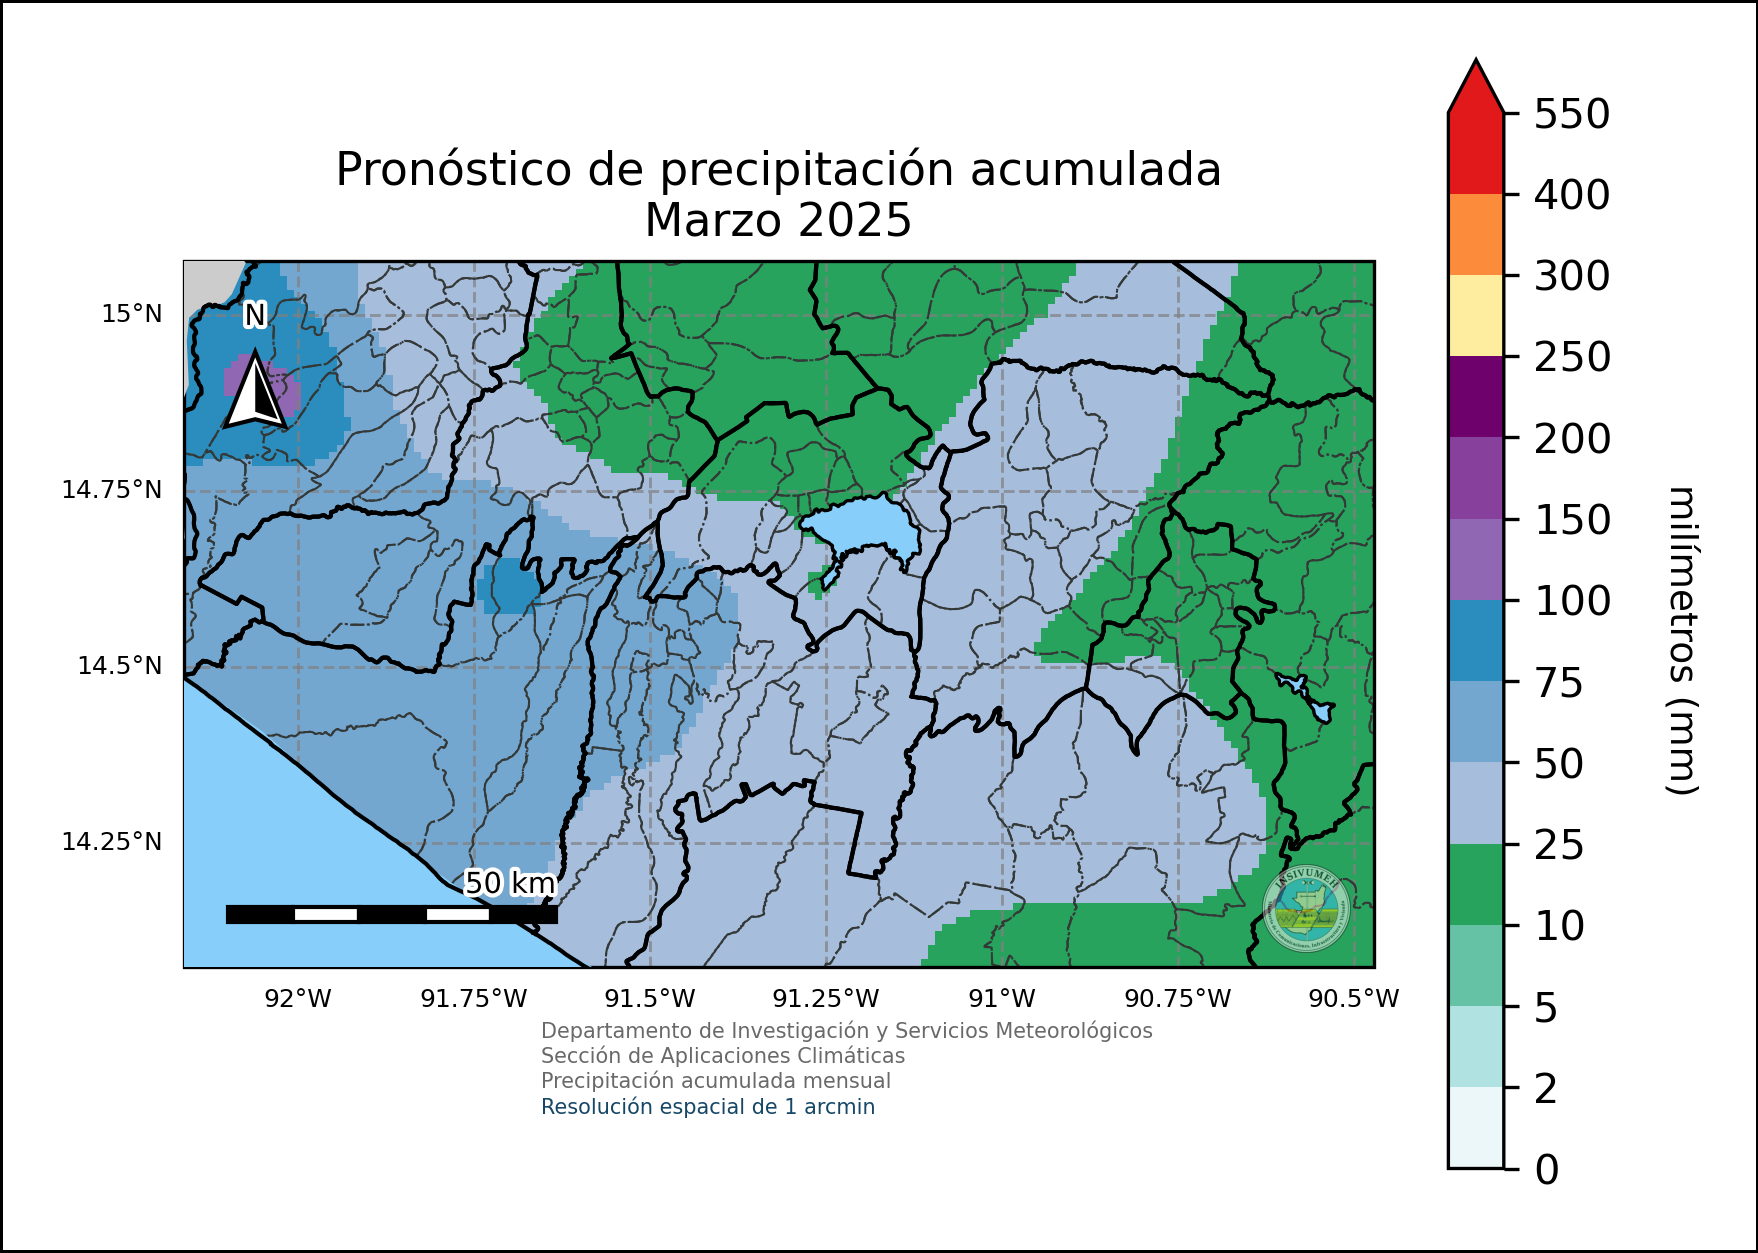
\includegraphics[width=\textwidth]{Informe/resultados/pronósticos/Pronóstico_3_2025_Boca Costa_03.png}
        \caption{Pronóstico de precipitación acumulada para el mes de marzo de 2025 dado por la LSTM.}
        \label{fig:pronosticolstm2503}
    \end{subfigure}
    \hfill
    \begin{subfigure}[b]{0.45\textwidth}
        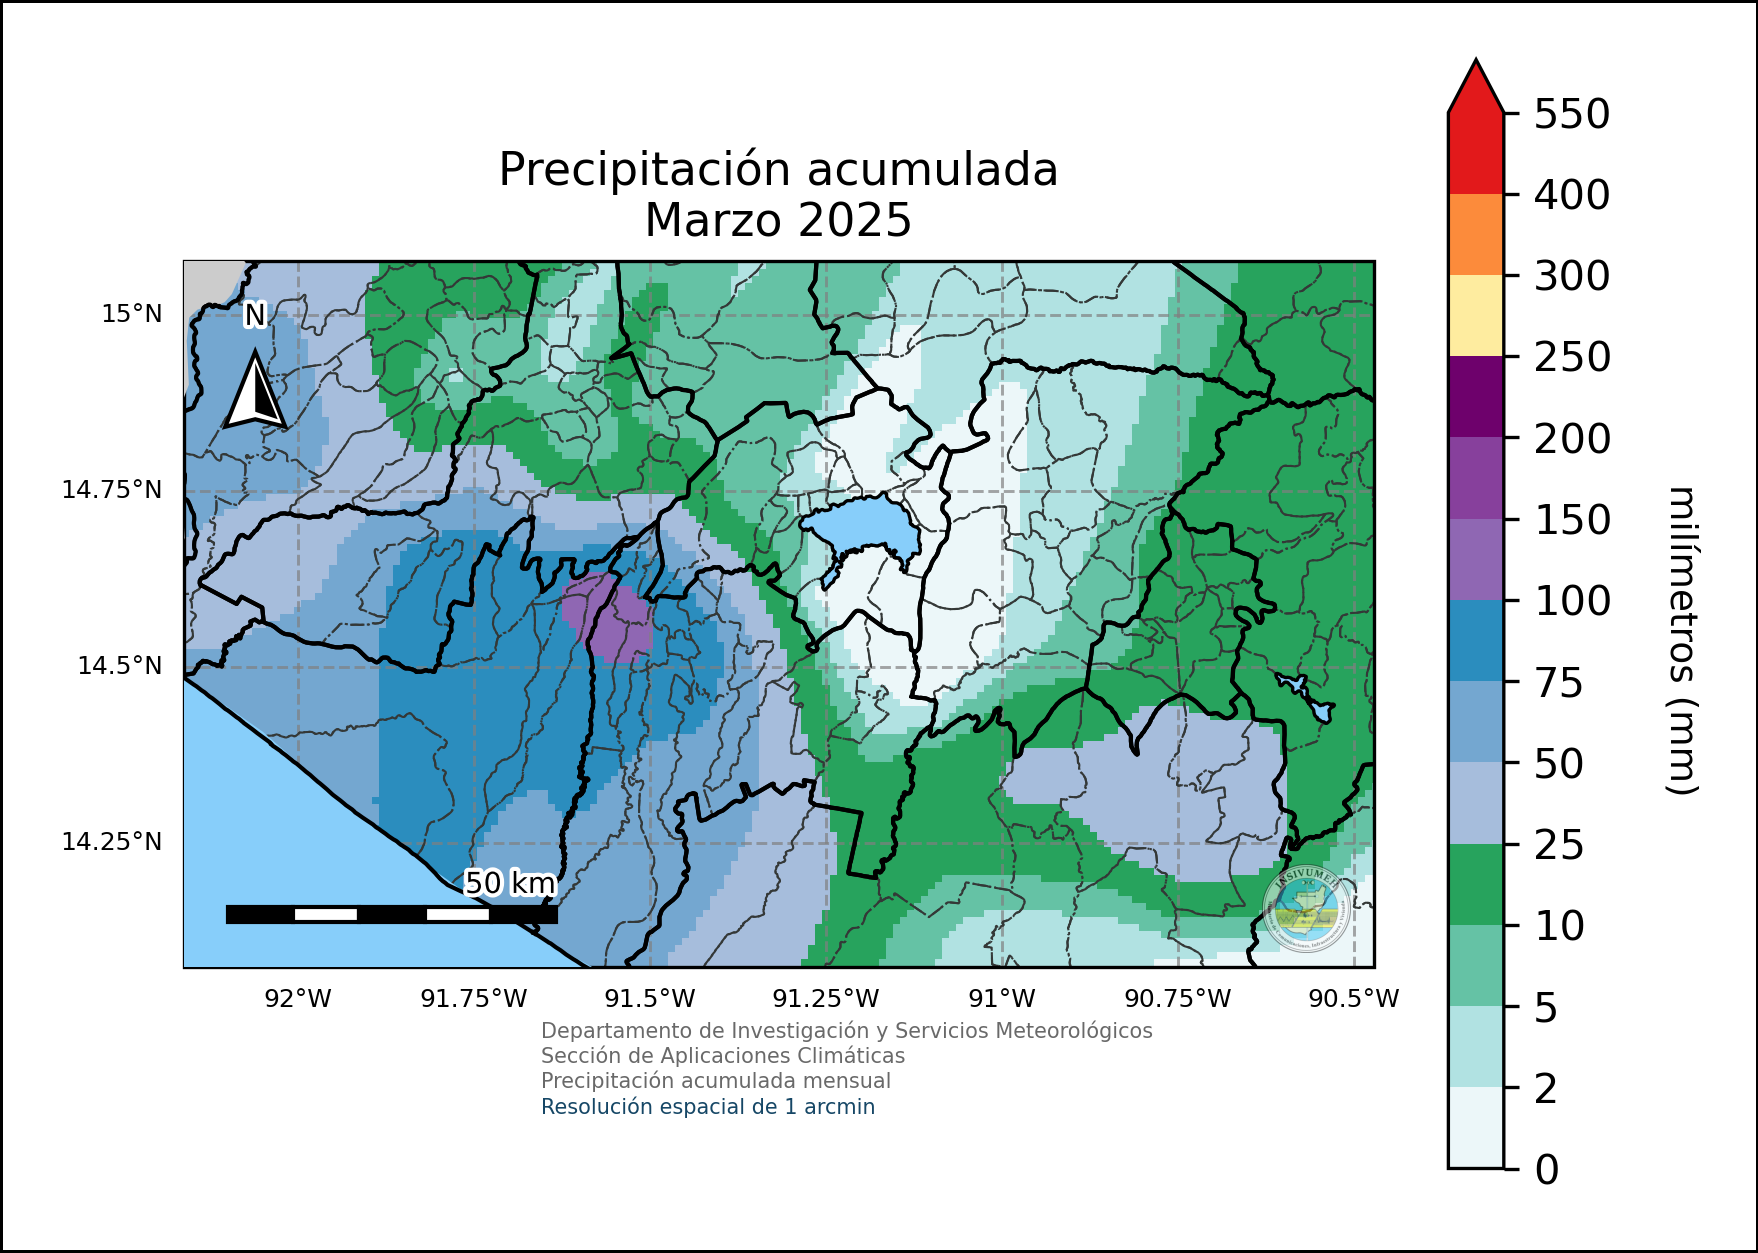
\includegraphics[width=\textwidth]{Informe/resultados/precipitación/Precipitación_3_2025_Boca Costa_03.png}
        \caption{Precipitación acumulada para el mes de marzo de 2025 dado por el registro de datos ENACTS.}
        \label{fig:precipenacts2503}
    \end{subfigure}
\end{figure}

% ========================= ABRIL =========================
\begin{figure}[H]
    \centering
    \begin{subfigure}[b]{0.45\textwidth}
        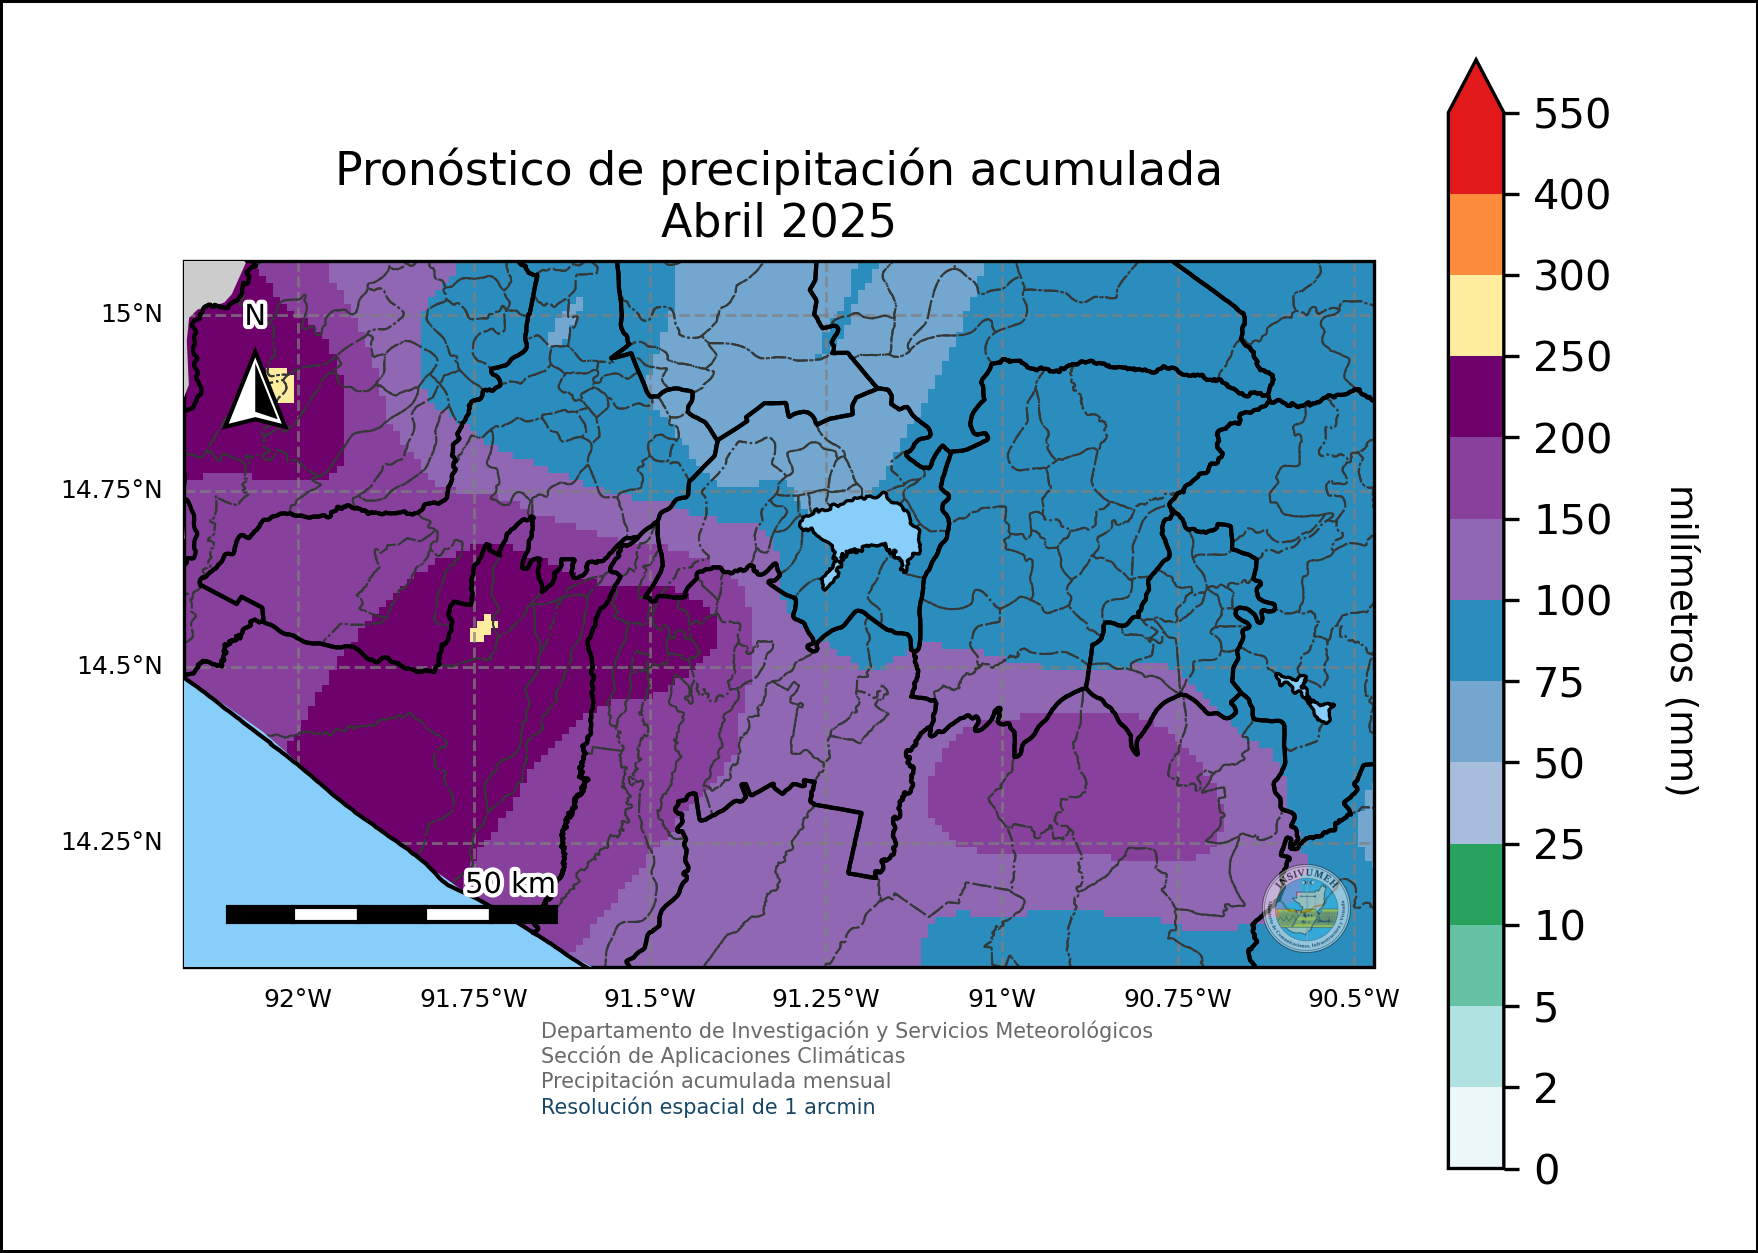
\includegraphics[width=\textwidth]{Informe/resultados/pronósticos/Pronóstico_4_2025_Boca Costa_03.png}
        \caption{Pronóstico de precipitación acumulada para el mes de abril de 2025 dado por la LSTM.}
        \label{fig:pronosticolstm2504}
    \end{subfigure}
    \hfill
    \begin{subfigure}[b]{0.45\textwidth}
        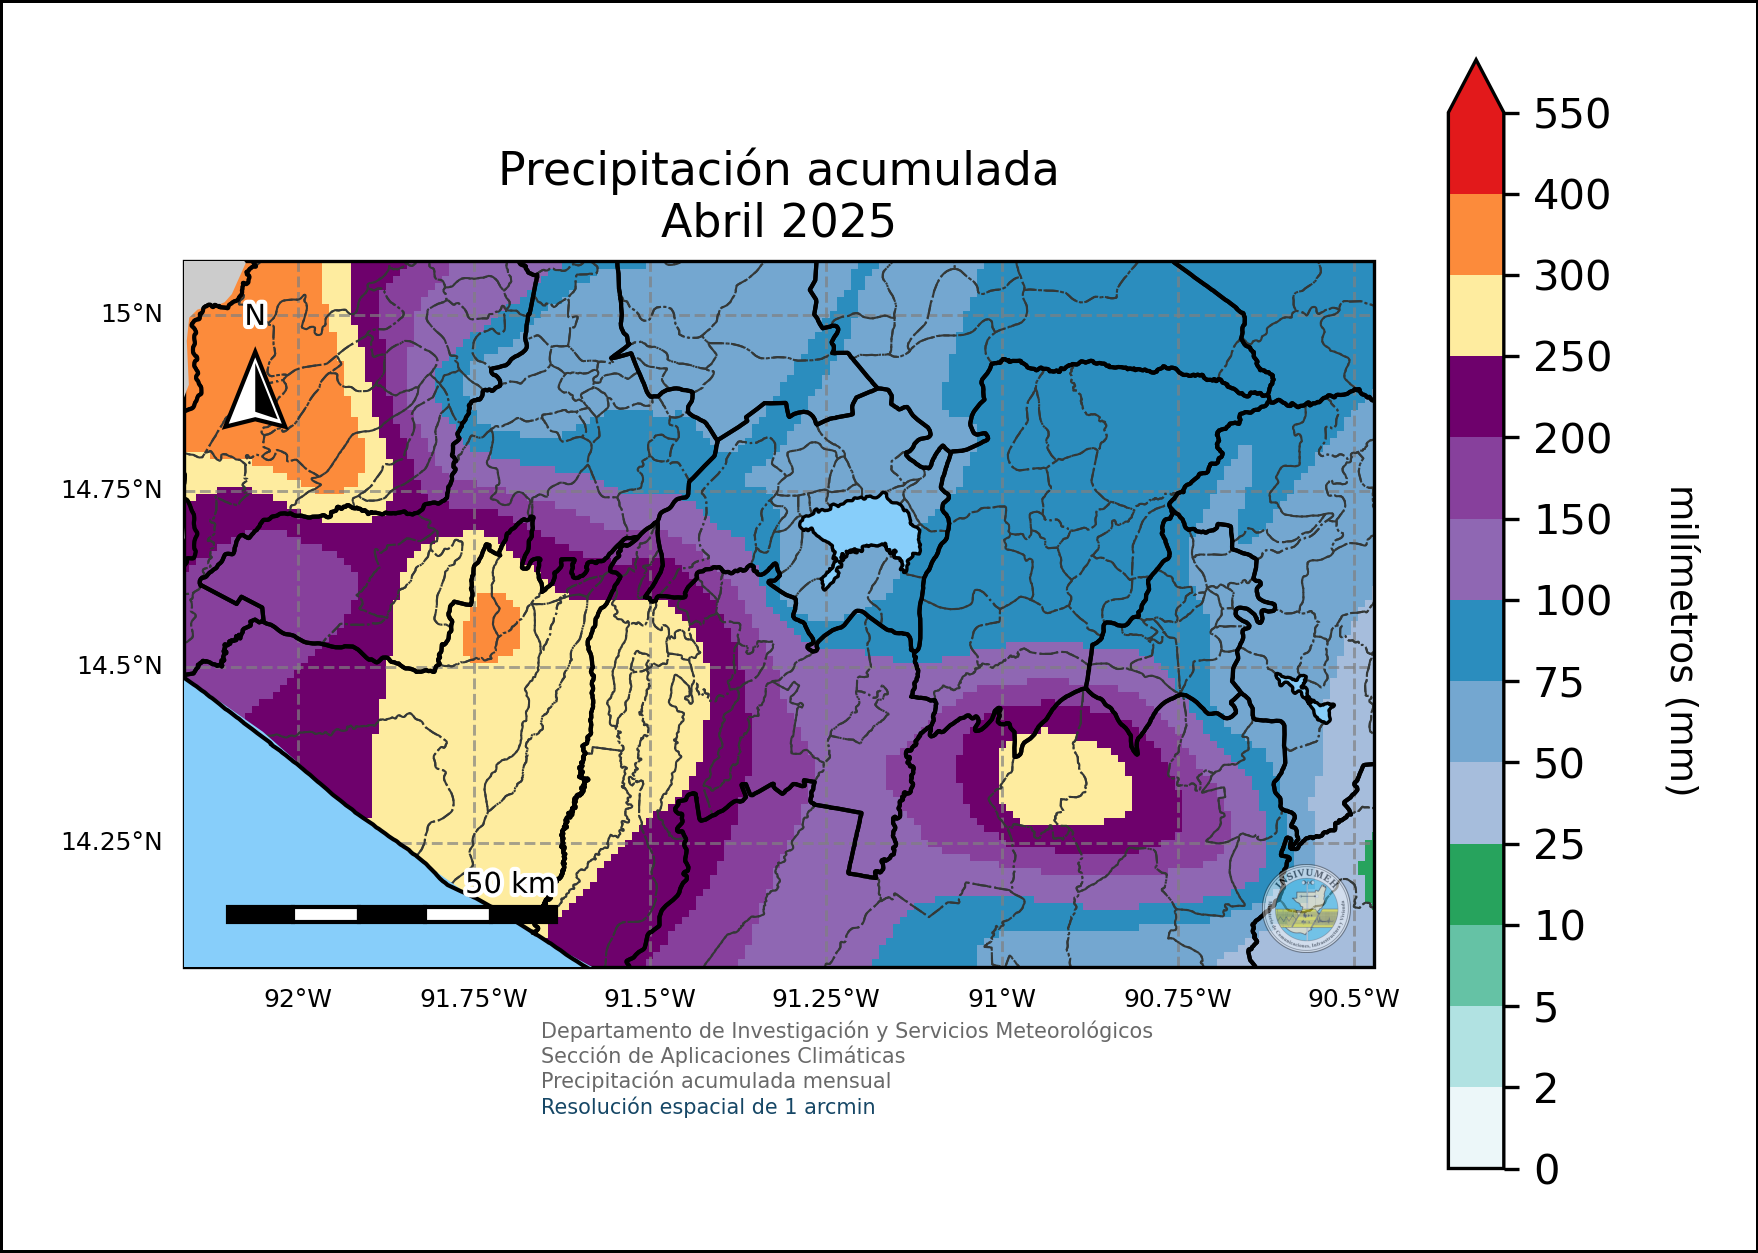
\includegraphics[width=\textwidth]{Informe/resultados/precipitación/Precipitación_4_2025_Boca Costa_03.png}
        \caption{Precipitación acumulada para el mes de abril de 2025 dado por el registro de datos ENACTS.}
        \label{fig:precipenacts2504}
    \end{subfigure}
\end{figure}

% ========================= MAYO =========================
\begin{figure}[H]
    \centering
    \begin{subfigure}[b]{0.45\textwidth}
        
\includegraphics[width=\textwidth]{Informe/resultados/pronósticos/Pronóstico_5_2025_Boca Costa_03.png}
        \caption{Pronóstico de precipitación acumulada para el mes de mayo de 2025 dado por la LSTM.}
        \label{fig:pronosticolstm2505}
    \end{subfigure}
    \hfill
    \begin{subfigure}[b]{0.45\textwidth}
        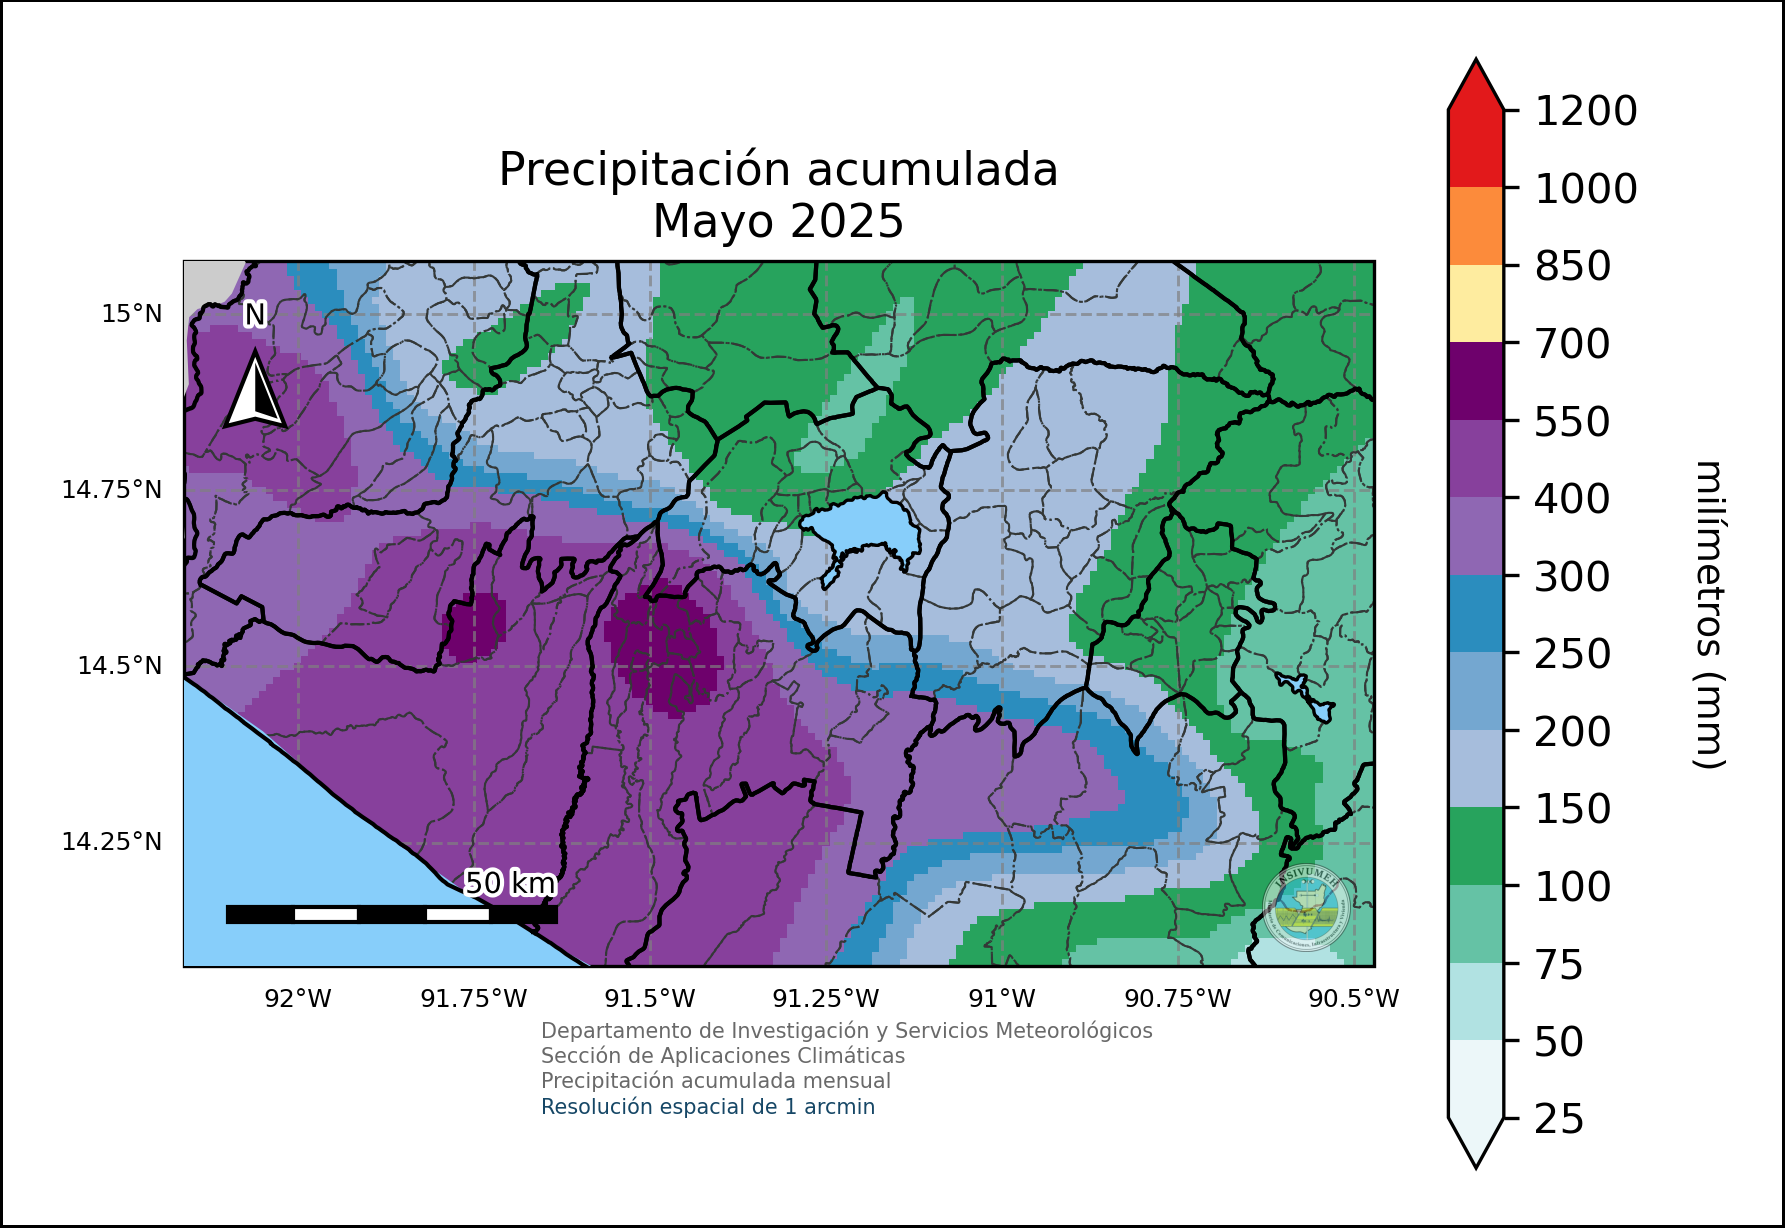
\includegraphics[width=\textwidth]{Informe/resultados/precipitación/Precipitación_5_2025_Boca Costa_03.png}
        \caption{Precipitación acumulada para el mes de mayo de 2025 dado por el registro de datos ENACTS.}
        \label{fig:precipenacts2505}
    \end{subfigure}
\end{figure}

% ========================= JUNIO =========================
\begin{figure}[H]
    \centering
    \begin{subfigure}[b]{0.45\textwidth}
        
\includegraphics[width=\textwidth]{Informe/resultados/pronósticos/Pronóstico_6_2025_Boca Costa_03.png}
        \caption{Pronóstico de precipitación acumulada para el mes de junio de 2025 dado por la LSTM.}
        \label{fig:pronosticolstm2506}
    \end{subfigure}
    \hfill
    \begin{subfigure}[b]{0.45\textwidth}
        
\includegraphics[width=\textwidth]{Informe/resultados/precipitación/Precipitación_6_2025_Boca Costa_03.png}
        \caption{Precipitación acumulada para el mes de junio de 2025 dado por el registro de datos ENACTS.}
        \label{fig:precipenacts2506}
    \end{subfigure}
\end{figure}

% ========================= JULIO =========================
\begin{figure}[H]
    \centering
    \begin{subfigure}[b]{0.45\textwidth}
        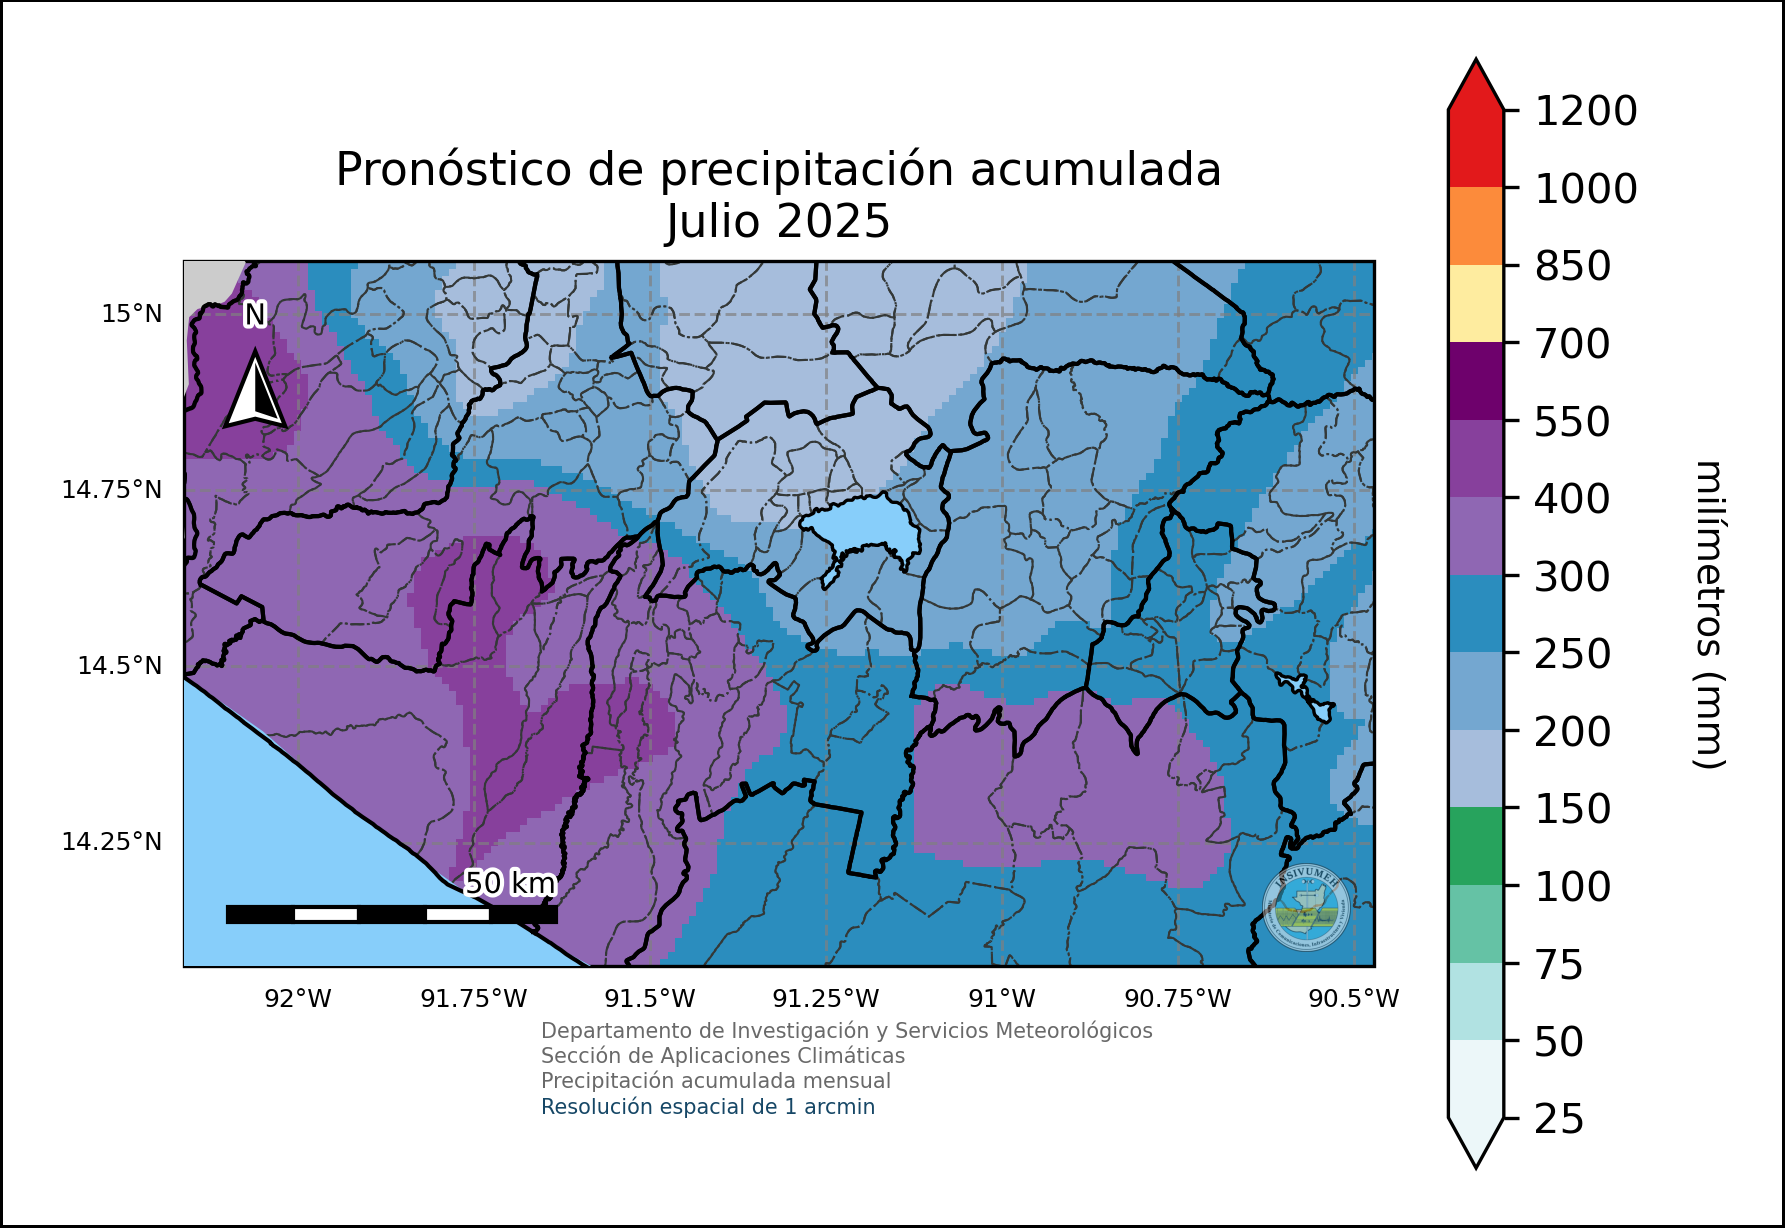
\includegraphics[width=\textwidth]{Informe/resultados/pronósticos/Pronóstico_7_2025_Boca Costa_03.png}
        \caption{Pronóstico de precipitación acumulada para el mes de julio de 2025 dado por la LSTM.}
        \label{fig:pronosticolstm2507}
    \end{subfigure}
    \hfill
    \begin{subfigure}[b]{0.45\textwidth}
        
\includegraphics[width=\textwidth]{Informe/resultados/precipitación/Precipitación_7_2025_Boca Costa_03.png}
        \caption{Precipitación acumulada para el mes de julio de 2025 dado por el registro de datos ENACTS.}
        \label{fig:precipenacts2507}
    \end{subfigure}
\end{figure}

% ========================= AGOSTO =========================
\begin{figure}[H]
    \centering
    \begin{subfigure}[b]{0.45\textwidth}
        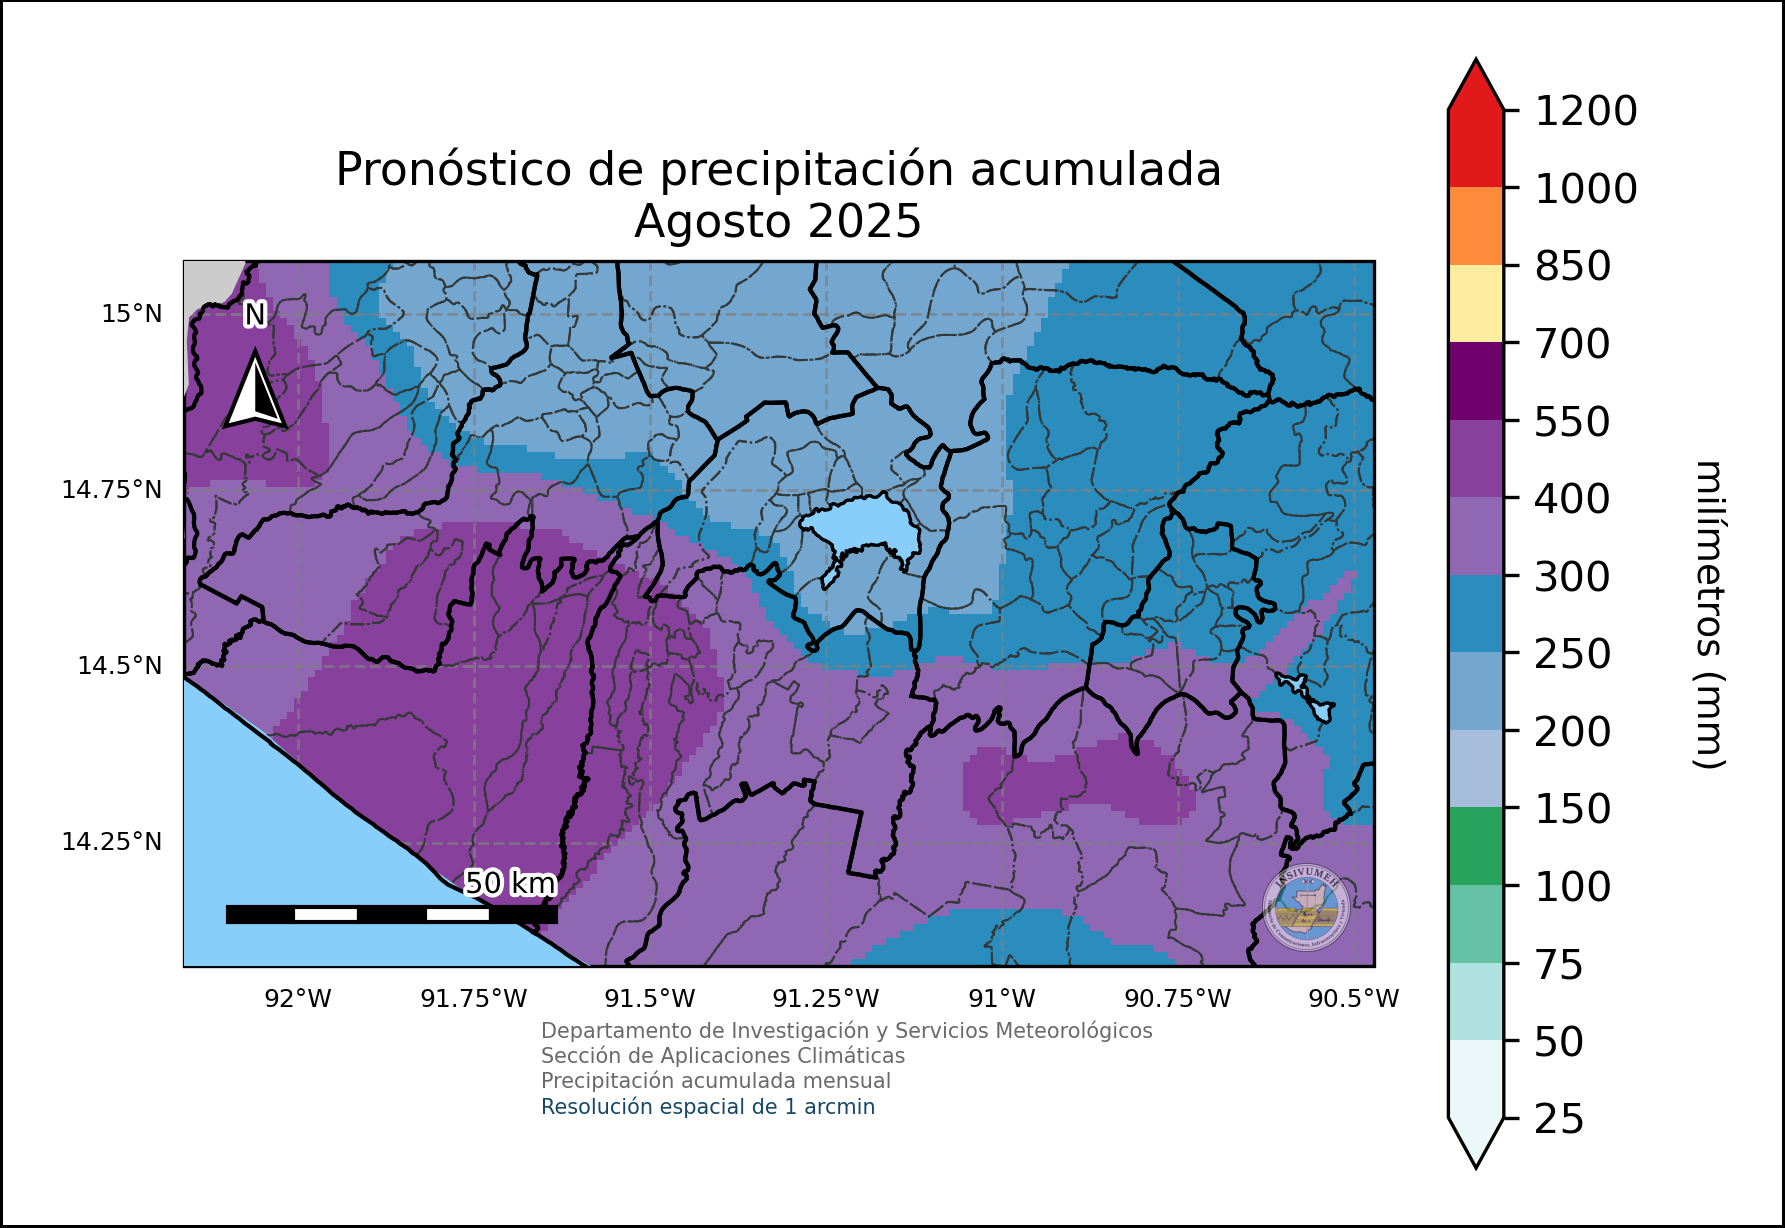
\includegraphics[width=\textwidth]{Informe/resultados/pronósticos/Pronóstico_8_2025_Boca Costa_03.png}
        \caption{Pronóstico de precipitación acumulada para el mes de agosto de 2025 dado por la LSTM.}
        \label{fig:pronosticolstm2508}
    \end{subfigure}
    \hfill
    \begin{subfigure}[b]{0.45\textwidth}
        
\includegraphics[width=\textwidth]{Informe/resultados/precipitación/Precipitación_8_2025_Boca Costa_03.png}
        \caption{Precipitación acumulada para el mes de agosto de 2025 dado por el registro de datos ENACTS.}
        \label{fig:precipenacts2508}
    \end{subfigure}
\end{figure}

% ========================= SEPTIEMBRE =========================
\begin{figure}[H]
    \centering
    \begin{subfigure}[b]{0.45\textwidth}
        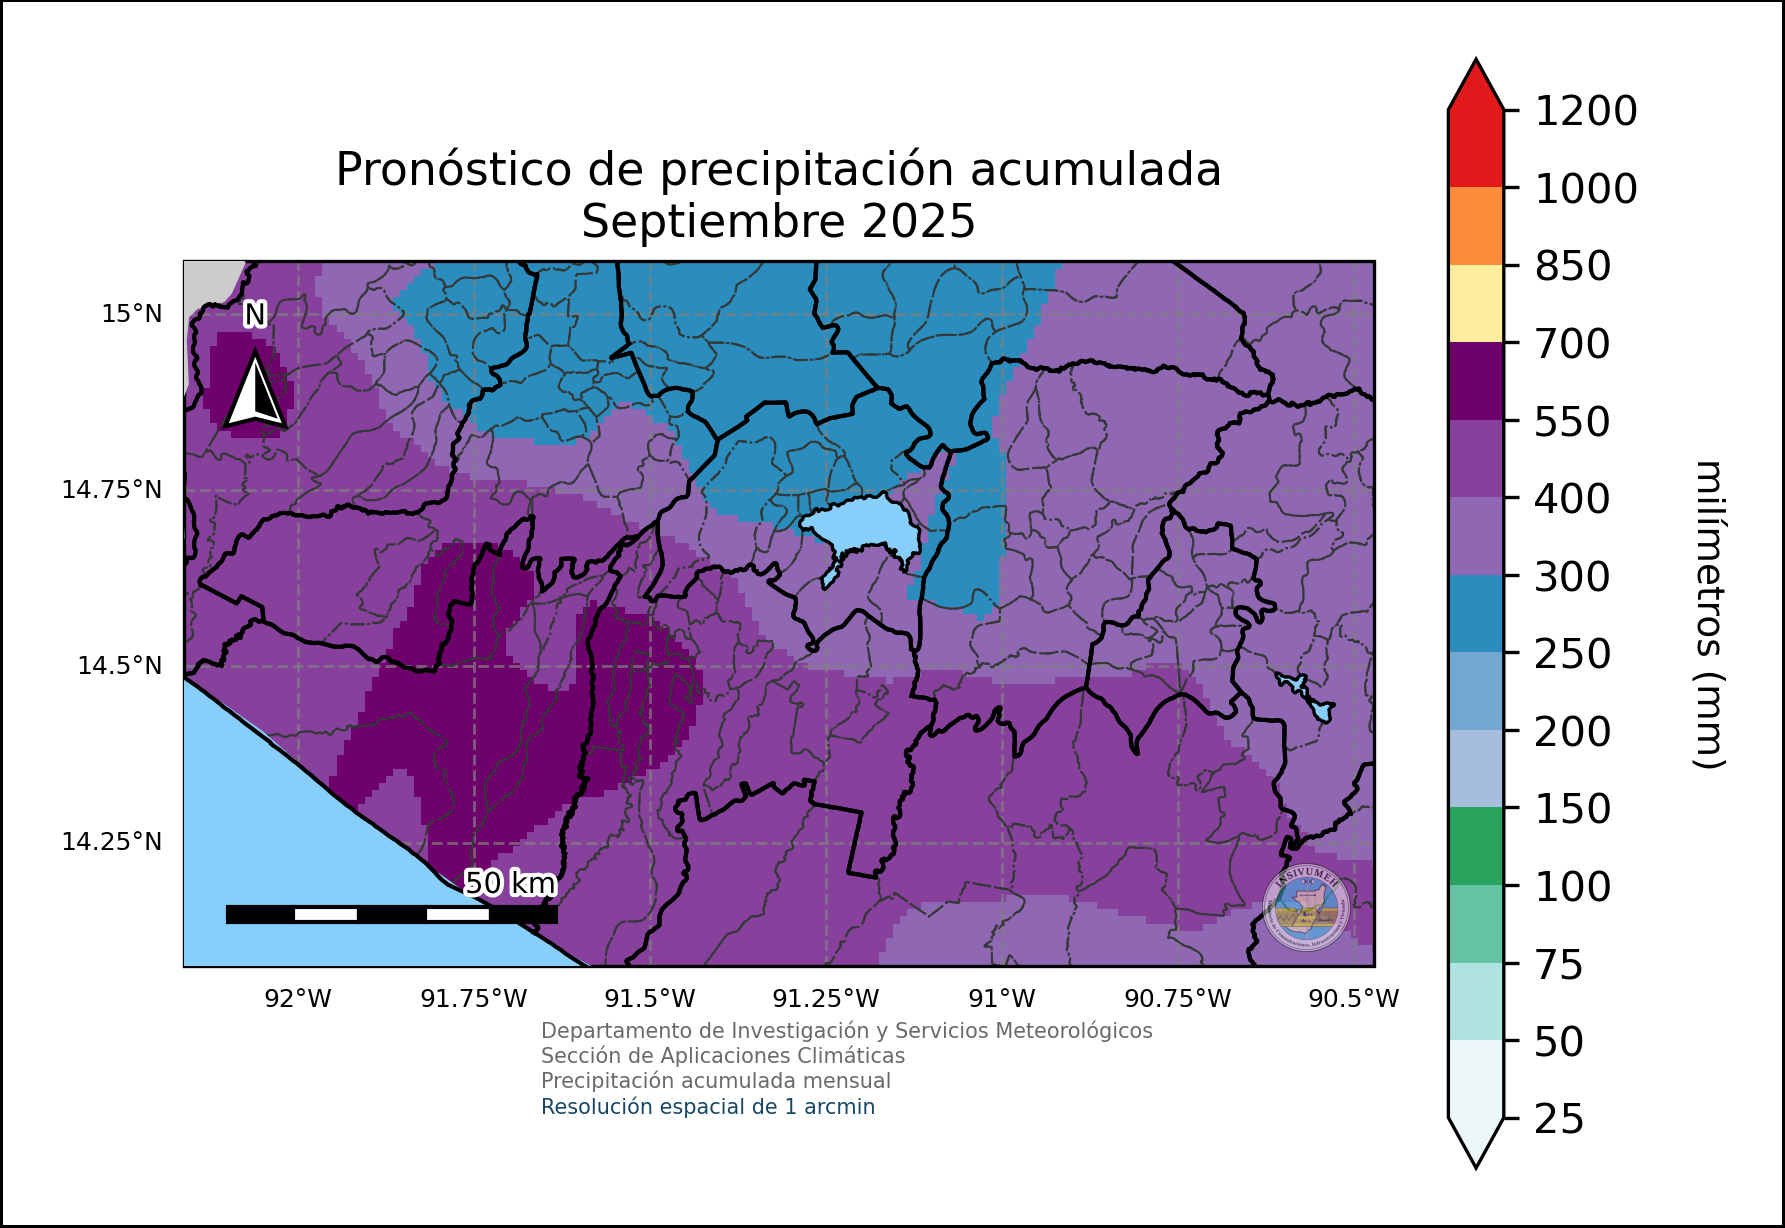
\includegraphics[width=\textwidth]{Informe/resultados/pronósticos/Pronóstico_9_2025_Boca Costa_03.png}
        \caption{Pronóstico de precipitación acumulada para el mes de septiembre de 2025 dado por la LSTM.}
        \label{fig:pronosticolstm2509}
    \end{subfigure}
    \hfill
    \begin{subfigure}[b]{0.45\textwidth}
        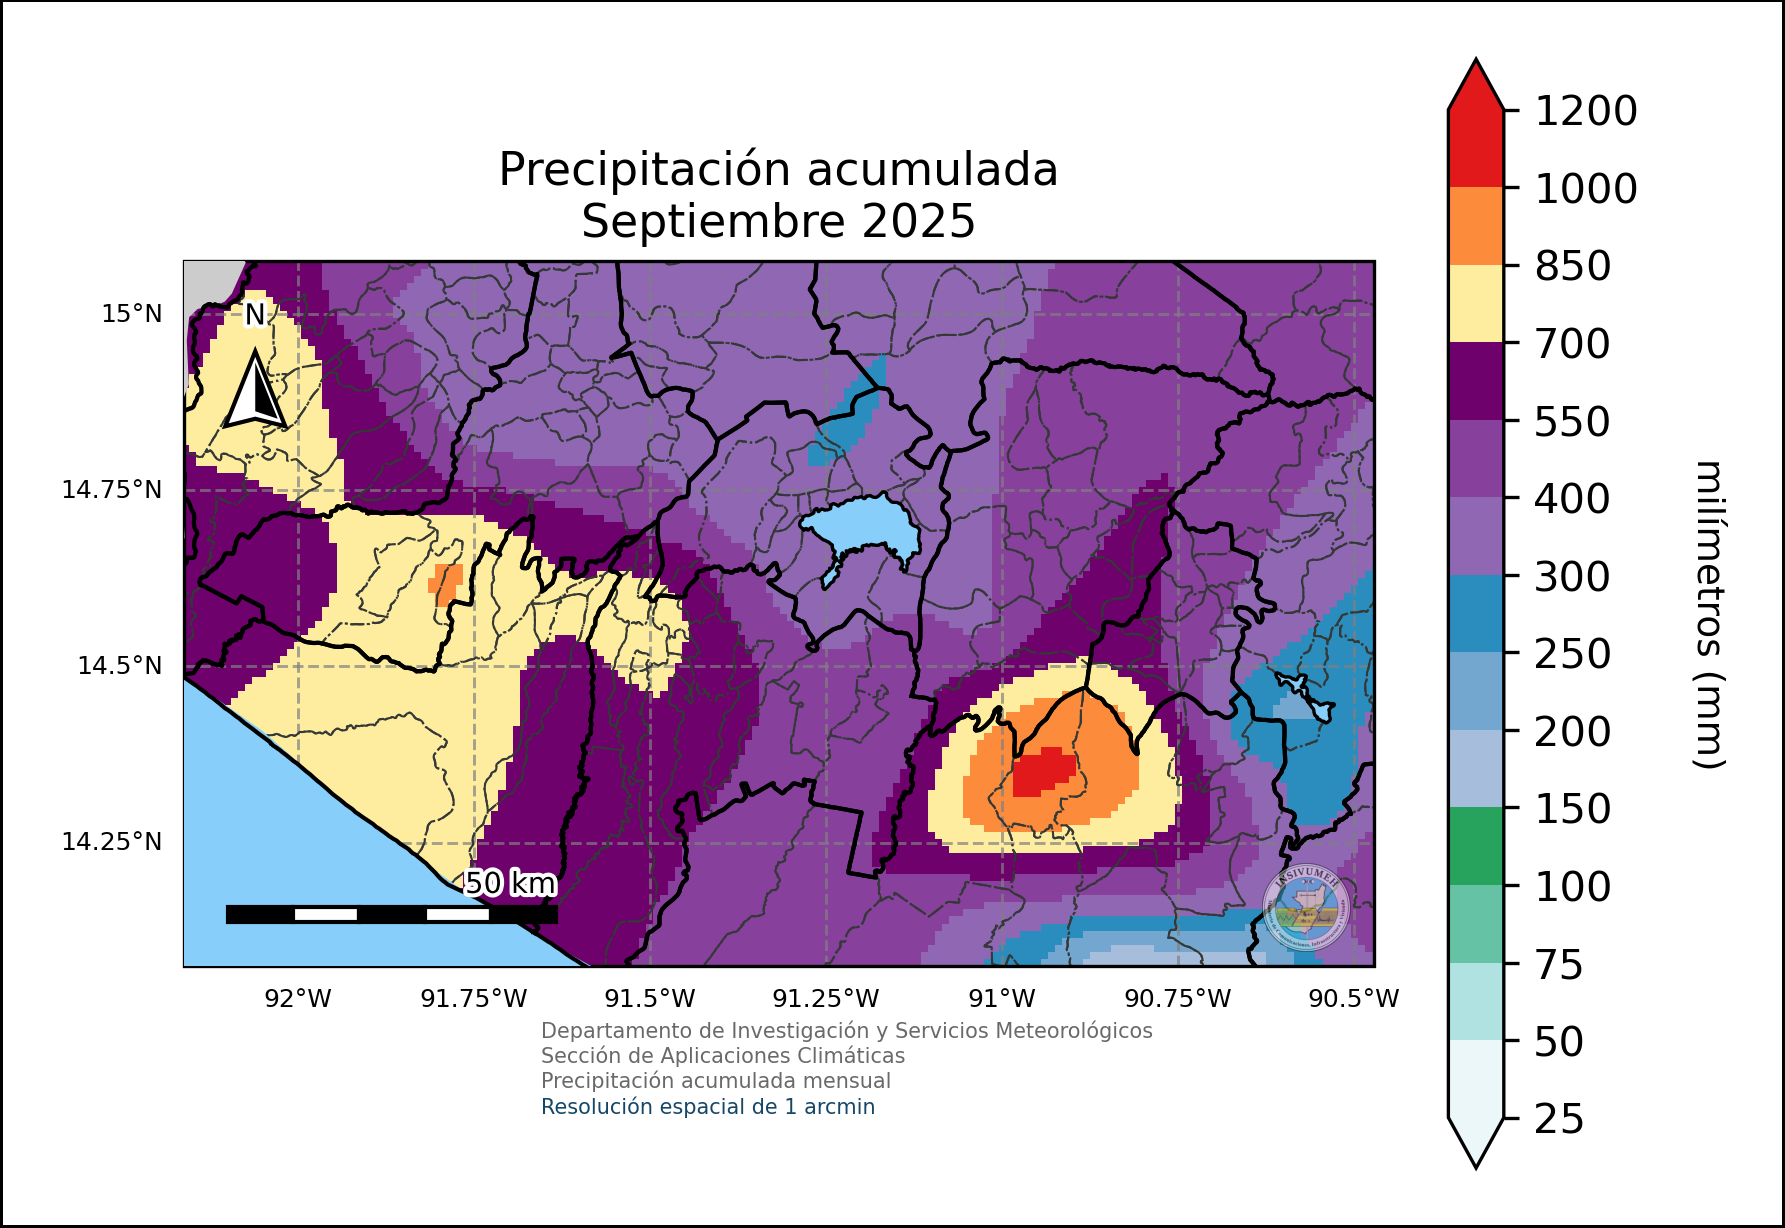
\includegraphics[width=\textwidth]{Informe/resultados/precipitación/Precipitación_9_2025_Boca Costa_03.png}
        \caption{Precipitación acumulada para el mes de septiembre de 2025 dado por el registro de datos ENACTS.}
        \label{fig:precipenacts2509}
    \end{subfigure}
\end{figure}

% ========================= OCTUBRE =========================
\begin{figure}[H]
    \centering
    \begin{subfigure}[b]{0.45\textwidth}
        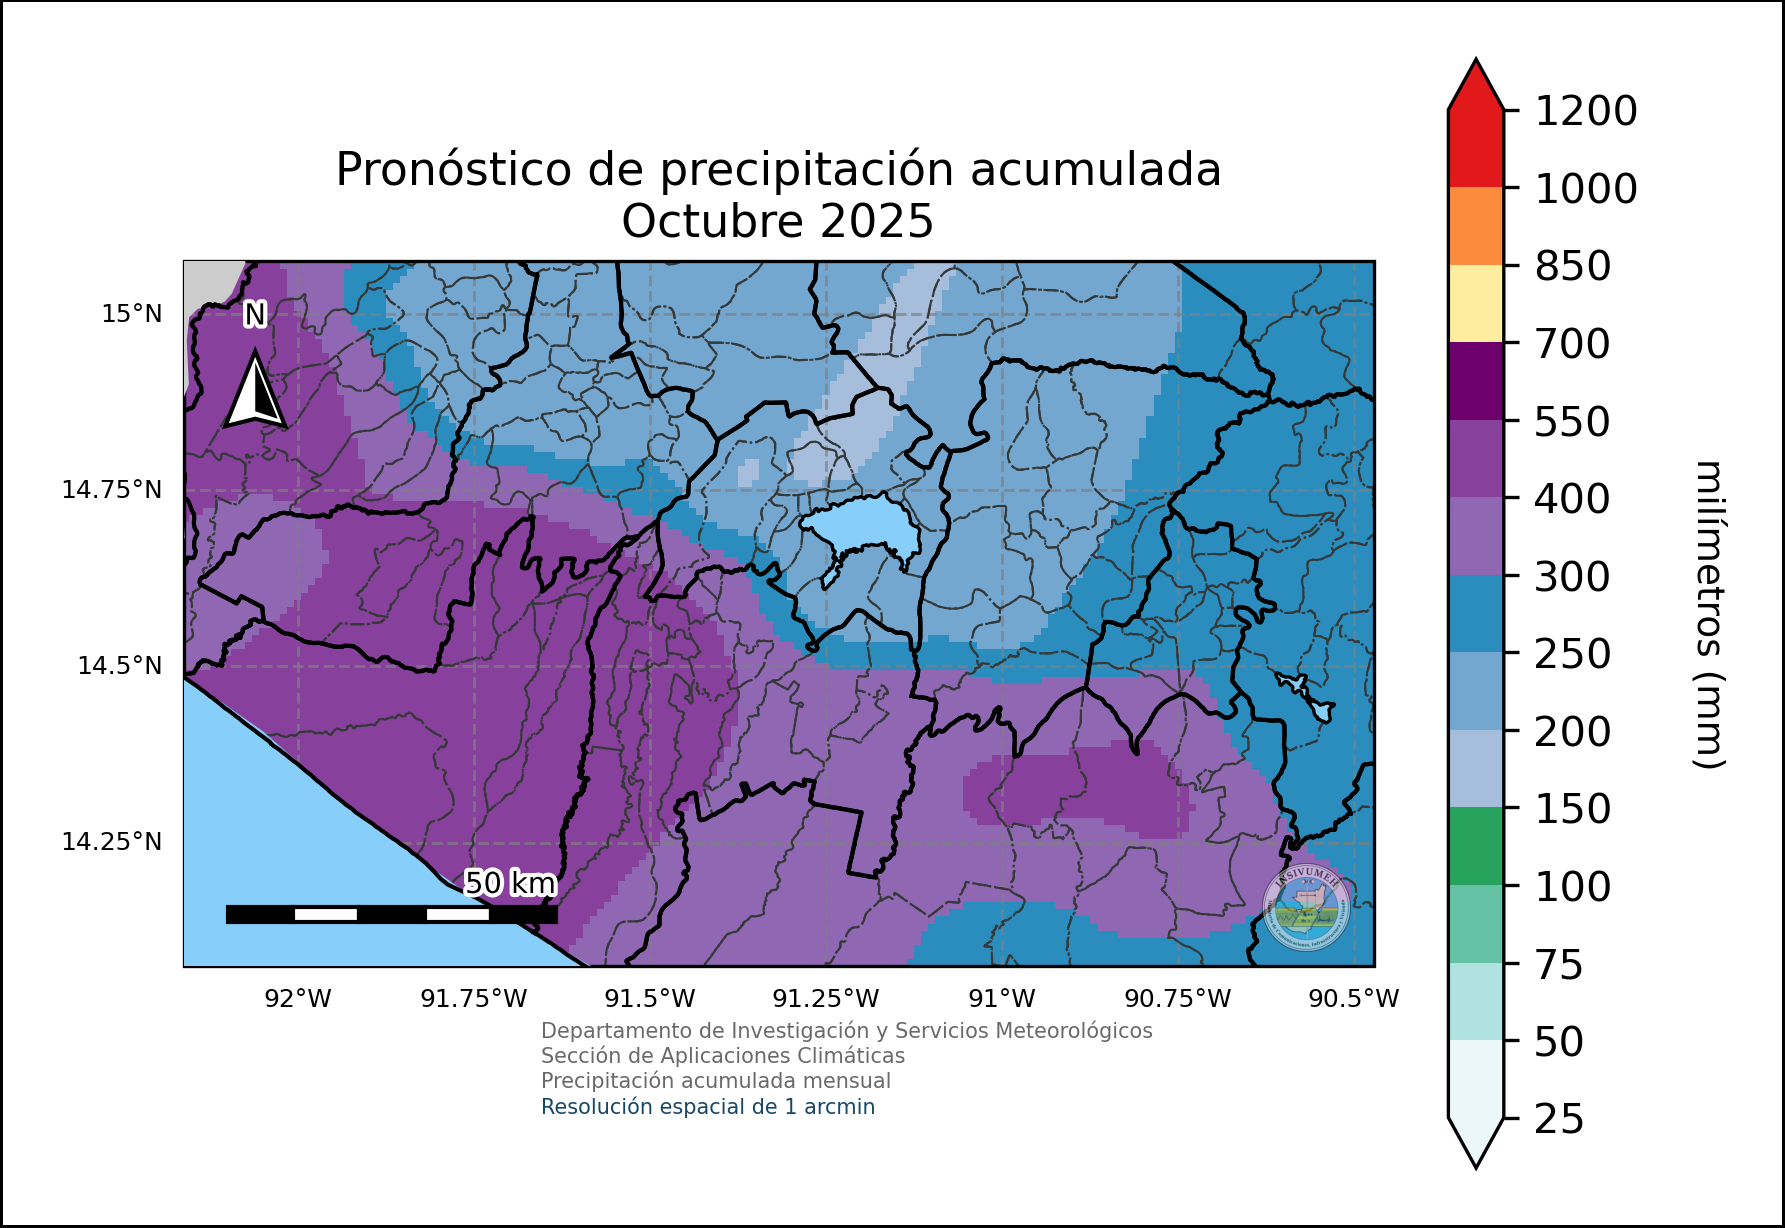
\includegraphics[width=\textwidth]{Informe/resultados/pronósticos/Pronóstico_10_2025_Boca Costa_03.png}
        \caption{Pronóstico de precipitación acumulada para el mes de octubre de 2025 dado por la LSTM.}
        \label{fig:pronosticolstm2510}
    \end{subfigure}
    \hfill
    \begin{subfigure}[b]{0.45\textwidth}
        
\includegraphics[width=\textwidth]{Informe/resultados/precipitación/Precipitación_10_2025_Boca Costa_03.png}
        \caption{Precipitación acumulada para el mes de octubre de 2025 dado por el registro de datos ENACTS.}
        \label{fig:precipenacts2510}
    \end{subfigure}
\end{figure}

% ========================= NOVIEMBRE =========================
\begin{figure}[H]
    \centering
    \begin{subfigure}[b]{0.45\textwidth}
        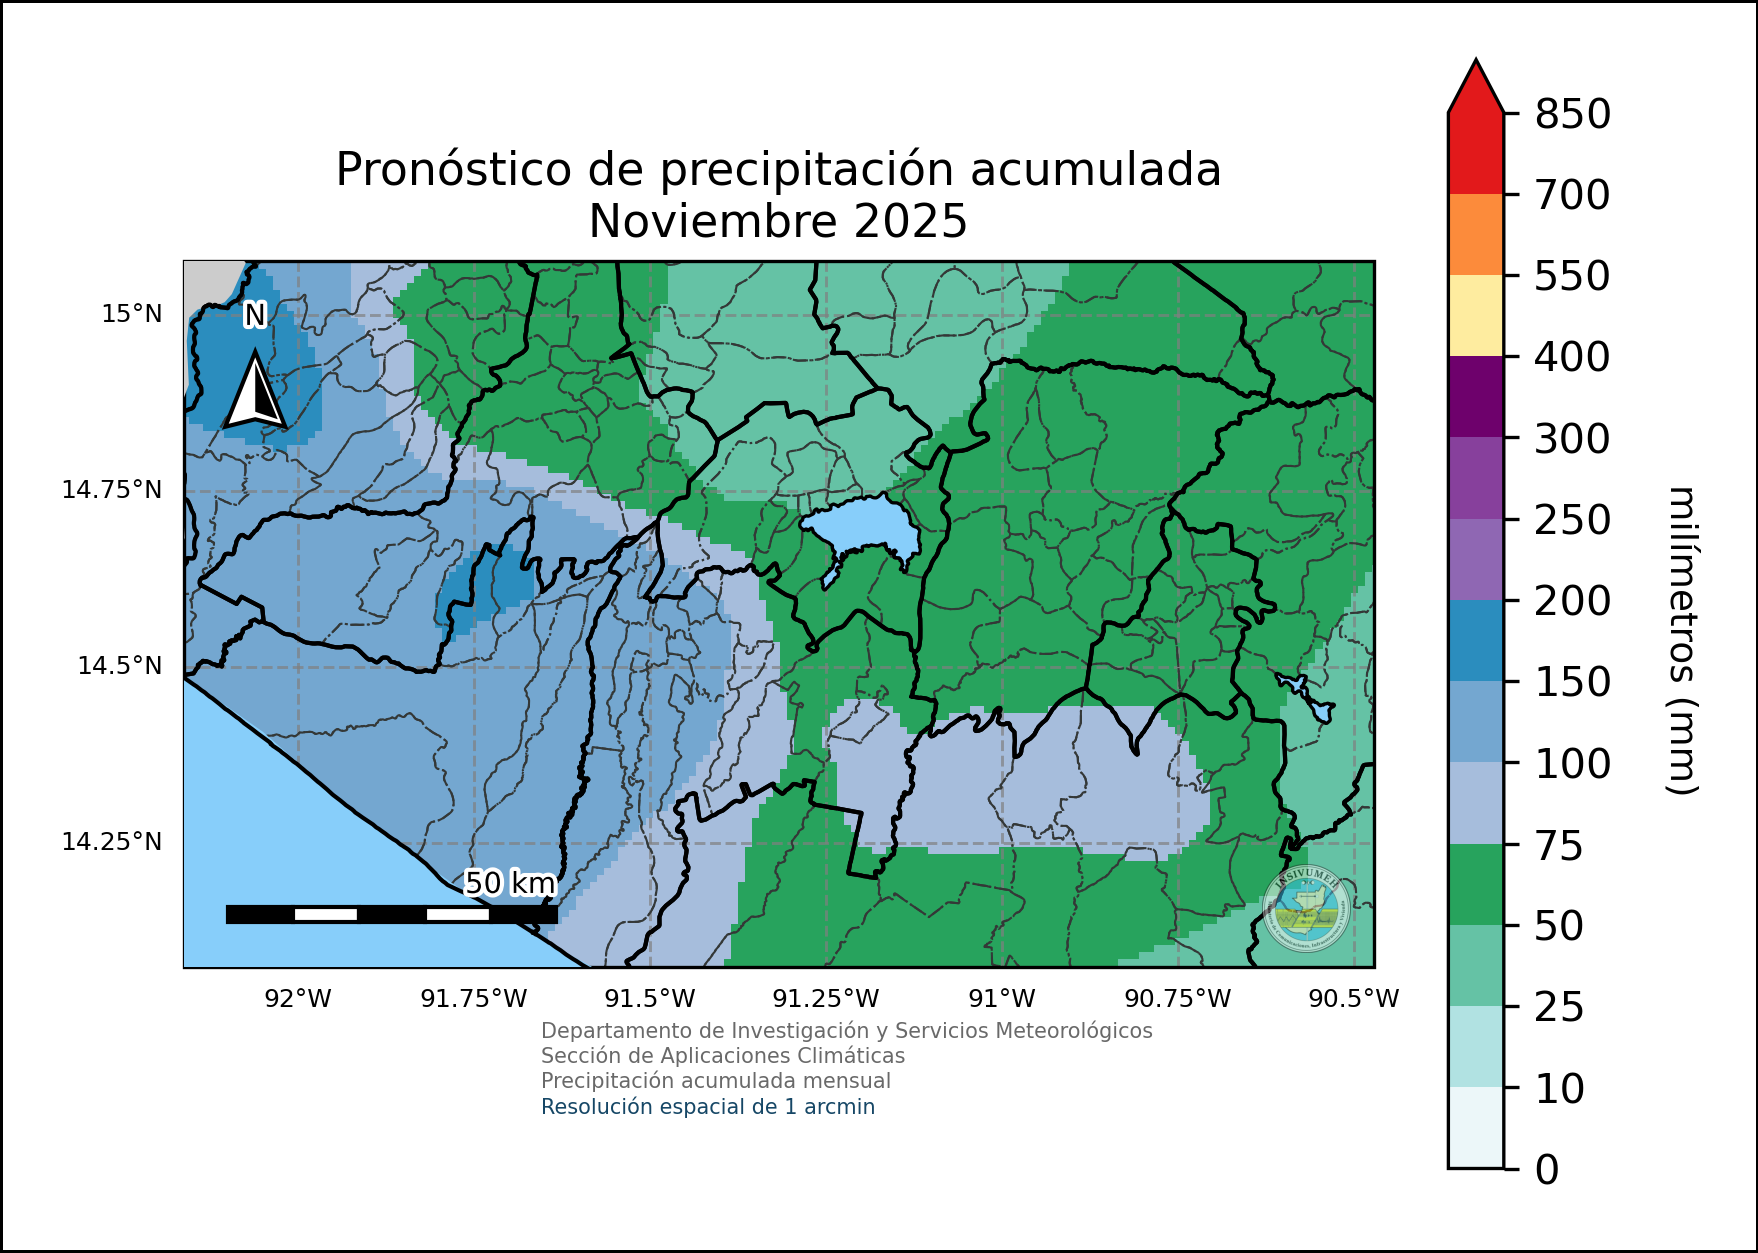
\includegraphics[width=\textwidth]{Informe/resultados/pronósticos/Pronóstico_11_2025_Boca Costa_03.png}
        \caption{Pronóstico de precipitación acumulada para el mes de noviembre de 2025 dado por la LSTM.}
        \label{fig:pronosticolstm2511}
    \end{subfigure}
    \hfill
    \begin{subfigure}[b]{0.45\textwidth}
        
\includegraphics[width=\textwidth]{Informe/resultados/precipitación/Precipitación_11_2025_Boca Costa_03.png}
        \caption{Precipitación acumulada para el mes de noviembre de 2025 dado por el registro de datos ENACTS.}
        \label{fig:precipenacts2511}
    \end{subfigure}
\end{figure}

% ========================= DICIEMBRE =========================
\begin{figure}[H]
    \centering
    \begin{subfigure}[b]{0.45\textwidth}
        
\includegraphics[width=\textwidth]{Informe/resultados/pronósticos/Pronóstico_12_2025_Boca Costa_03.png}
        \caption{Pronóstico de precipitación acumulada para el mes de diciembre de 2025 dado por la LSTM.}
        \label{fig:pronosticolstm2512}
    \end{subfigure}
    \hfill
    \begin{subfigure}[b]{0.45\textwidth}
        
\includegraphics[width=\textwidth]{Informe/resultados/precipitación/Precipitación_12_2025_Boca Costa_03.png}
        \caption{Precipitación acumulada para el mes de diciembre de 2025 dado por el registro de datos ENACTS.}
        \label{fig:precipenacts2512}
    \end{subfigure}
\end{figure}